% Options for packages loaded elsewhere
\PassOptionsToPackage{unicode}{hyperref}
\PassOptionsToPackage{hyphens}{url}
\PassOptionsToPackage{dvipsnames,svgnames,x11names}{xcolor}
%
\documentclass[
]{article}
\usepackage{amsmath,amssymb}
\usepackage{iftex}
\ifPDFTeX
  \usepackage[T1]{fontenc}
  \usepackage[utf8]{inputenc}
  \usepackage{textcomp} % provide euro and other symbols
\else % if luatex or xetex
  \usepackage{unicode-math} % this also loads fontspec
  \defaultfontfeatures{Scale=MatchLowercase}
  \defaultfontfeatures[\rmfamily]{Ligatures=TeX,Scale=1}
\fi
\usepackage{lmodern}
\ifPDFTeX\else
  % xetex/luatex font selection
\fi
% Use upquote if available, for straight quotes in verbatim environments
\IfFileExists{upquote.sty}{\usepackage{upquote}}{}
\IfFileExists{microtype.sty}{% use microtype if available
  \usepackage[]{microtype}
  \UseMicrotypeSet[protrusion]{basicmath} % disable protrusion for tt fonts
}{}
\makeatletter
\@ifundefined{KOMAClassName}{% if non-KOMA class
  \IfFileExists{parskip.sty}{%
    \usepackage{parskip}
  }{% else
    \setlength{\parindent}{0pt}
    \setlength{\parskip}{6pt plus 2pt minus 1pt}}
}{% if KOMA class
  \KOMAoptions{parskip=half}}
\makeatother
\usepackage{xcolor}
\usepackage{longtable,booktabs,array}
\usepackage{calc} % for calculating minipage widths
% Correct order of tables after \paragraph or \subparagraph
\usepackage{etoolbox}
\makeatletter
\patchcmd\longtable{\par}{\if@noskipsec\mbox{}\fi\par}{}{}
\makeatother
% Allow footnotes in longtable head/foot
\IfFileExists{footnotehyper.sty}{\usepackage{footnotehyper}}{\usepackage{footnote}}
\makesavenoteenv{longtable}
\usepackage{graphicx}
\makeatletter
\def\maxwidth{\ifdim\Gin@nat@width>\linewidth\linewidth\else\Gin@nat@width\fi}
\def\maxheight{\ifdim\Gin@nat@height>\textheight\textheight\else\Gin@nat@height\fi}
\makeatother
% Scale images if necessary, so that they will not overflow the page
% margins by default, and it is still possible to overwrite the defaults
% using explicit options in \includegraphics[width, height, ...]{}
\setkeys{Gin}{width=\maxwidth,height=\maxheight,keepaspectratio}
% Set default figure placement to htbp
\makeatletter
\def\fps@figure{htbp}
\makeatother
\usepackage{svg}
\setlength{\emergencystretch}{3em} % prevent overfull lines
\providecommand{\tightlist}{%
  \setlength{\itemsep}{0pt}\setlength{\parskip}{0pt}}
\setcounter{secnumdepth}{5}
% definitions for citeproc citations
\NewDocumentCommand\citeproctext{}{}
\NewDocumentCommand\citeproc{mm}{%
  \begingroup\def\citeproctext{#2}\cite{#1}\endgroup}
\makeatletter
 % allow citations to break across lines
 \let\@cite@ofmt\@firstofone
 % avoid brackets around text for \cite:
 \def\@biblabel#1{}
 \def\@cite#1#2{{#1\if@tempswa , #2\fi}}
\makeatother
\newlength{\cslhangindent}
\setlength{\cslhangindent}{1.5em}
\newlength{\csllabelwidth}
\setlength{\csllabelwidth}{3em}
\newenvironment{CSLReferences}[2] % #1 hanging-indent, #2 entry-spacing
 {\begin{list}{}{%
  \setlength{\itemindent}{0pt}
  \setlength{\leftmargin}{0pt}
  \setlength{\parsep}{0pt}
  % turn on hanging indent if param 1 is 1
  \ifodd #1
   \setlength{\leftmargin}{\cslhangindent}
   \setlength{\itemindent}{-1\cslhangindent}
  \fi
  % set entry spacing
  \setlength{\itemsep}{#2\baselineskip}}}
 {\end{list}}
\usepackage{calc}
\newcommand{\CSLBlock}[1]{\hfill\break\parbox[t]{\linewidth}{\strut\ignorespaces#1\strut}}
\newcommand{\CSLLeftMargin}[1]{\parbox[t]{\csllabelwidth}{\strut#1\strut}}
\newcommand{\CSLRightInline}[1]{\parbox[t]{\linewidth - \csllabelwidth}{\strut#1\strut}}
\newcommand{\CSLIndent}[1]{\hspace{\cslhangindent}#1}
%% personal sizes for drafts
\topmargin=-0.5in
\textheight=9.2in
\oddsidemargin=-0.2in
\evensidemargin=0.0in
\textwidth=6.90in
\parindent=30pt
\parskip=3pt
\headheight=15pt
\reversemarginpar
\marginparwidth=.75in

%\setkeys{Gin}{width=.75\textwidth,keepaspectratio}


\makeatletter
\@ifpackageloaded{subfig}{}{\usepackage{subfig}}
\@ifpackageloaded{caption}{}{\usepackage{caption}}
\captionsetup[subfloat]{margin=0.5em}
\AtBeginDocument{%
\renewcommand*\figurename{Figure}
\renewcommand*\tablename{Table}
}
\AtBeginDocument{%
\renewcommand*\listfigurename{List of Figures}
\renewcommand*\listtablename{List of Tables}
}
\newcounter{pandoccrossref@subfigures@footnote@counter}
\newenvironment{pandoccrossrefsubfigures}{%
\setcounter{pandoccrossref@subfigures@footnote@counter}{0}
\begin{figure}\centering%
\gdef\global@pandoccrossref@subfigures@footnotes{}%
\DeclareRobustCommand{\footnote}[1]{\footnotemark%
\stepcounter{pandoccrossref@subfigures@footnote@counter}%
\ifx\global@pandoccrossref@subfigures@footnotes\empty%
\gdef\global@pandoccrossref@subfigures@footnotes{{##1}}%
\else%
\g@addto@macro\global@pandoccrossref@subfigures@footnotes{, {##1}}%
\fi}}%
{\end{figure}%
\addtocounter{footnote}{-\value{pandoccrossref@subfigures@footnote@counter}}
\@for\f:=\global@pandoccrossref@subfigures@footnotes\do{\stepcounter{footnote}\footnotetext{\f}}%
\gdef\global@pandoccrossref@subfigures@footnotes{}}
\@ifpackageloaded{float}{}{\usepackage{float}}
\floatstyle{ruled}
\@ifundefined{c@chapter}{\newfloat{codelisting}{h}{lop}}{\newfloat{codelisting}{h}{lop}[chapter]}
\floatname{codelisting}{Listing}
\newcommand*\listoflistings{\listof{codelisting}{List of Listings}}
\makeatother
\ifLuaTeX
  \usepackage{selnolig}  % disable illegal ligatures
\fi
\usepackage{bookmark}
\IfFileExists{xurl.sty}{\usepackage{xurl}}{} % add URL line breaks if available
\urlstyle{same}
\hypersetup{
  pdftitle={How to Apply BCM Theory: A Practical Guide Using Amblyopia Treatment as an Example},
  pdfkeywords={bcm, amblyopia, synaptic plasticity},
  colorlinks=true,
  linkcolor={Maroon},
  filecolor={Maroon},
  citecolor={Blue},
  urlcolor={Blue},
  pdfcreator={LaTeX via pandoc}}

\title{How to Apply BCM Theory: A Practical Guide Using Amblyopia
Treatment as an Example}
\author{}
\date{}

\begin{document}
\maketitle
\begin{abstract}
This document should serve as an introduction to the BCM
Theory\textsuperscript{1} of cortical plasticity, using the development
and treatment for amblyopia as the scientific problem to be explored. We
will explore both low-dimensional abstract environments as well as
visual environments based on natural-image input to understand the
dynamics of synaptic plasticity.
\end{abstract}

{
\hypersetup{linkcolor=}
\setcounter{tocdepth}{3}
\tableofcontents
}
\section{Introduction}\label{sec:introduction}

In this introduction, I want to be clear about as many of the underlying
assumptions being made and to highlight where the various results come
from in the simulations. By comparing low-dimension and high-dimension
environments, it's my hope that it will make clearer what sorts of
changes to the input environment will lead to particular dynamics of
synaptic plasticity. Building up one's intuition this way should help in
proposing alternate treatments for amblyopia and understanding how the
parameters of those treatments affect their outcomes.

\subsection{The Neuron}\label{sec:the-neuron}

The BCM theory\textsuperscript{1} of synaptic plasticity starts with a
simplified model of a neuron shown in Figure \ref{fig:simple_neuron}. In
the figure, the model of the neuron has 4 inputs denoted as
\(x_1, x_2, x_3,\) and \(x_4\). These inputs are connected to the cell
via 4 synaptic weights, denoted as \(w_1, w_2, w_3,\) and \(w_4\). The
output of the cell, \(y\), is given as a sum of the input values each
multiplied by the synaptic weight connecting it to the neuron passed
through an output function, often a sigmoid, \(\sigma\): \[
y=\sigma\left(\sum_i x_i w_i \right)
\] In this simple model, the value of neural activity \(x_i=0\) or
\(y=0\) refers to \emph{spontaneous activity}, thus one can have
negative values for this activity representing \emph{below spontaneous}
activity. The sigmoid function is chosen to have the effect of limiting
the spontaneous level of activity, i.e.~the neuron has a larger range of
activity above spontaneous than below it.

The synapse values, \(w_i\), may represent the combination of several
synapses -- including inhibitory synapses -- which implies that the
weights can take on both positive and negative values. The number of
inputs (4 in the case of Figure \ref{fig:simple_neuron}) is arbitrary
and will be different from one environment to another. What is called a
``low-dimensional'' environment is one with few inputs, likewise a
``high-dimensional'' environment will have many (possibly hundreds).

\begin{figure}
\centering
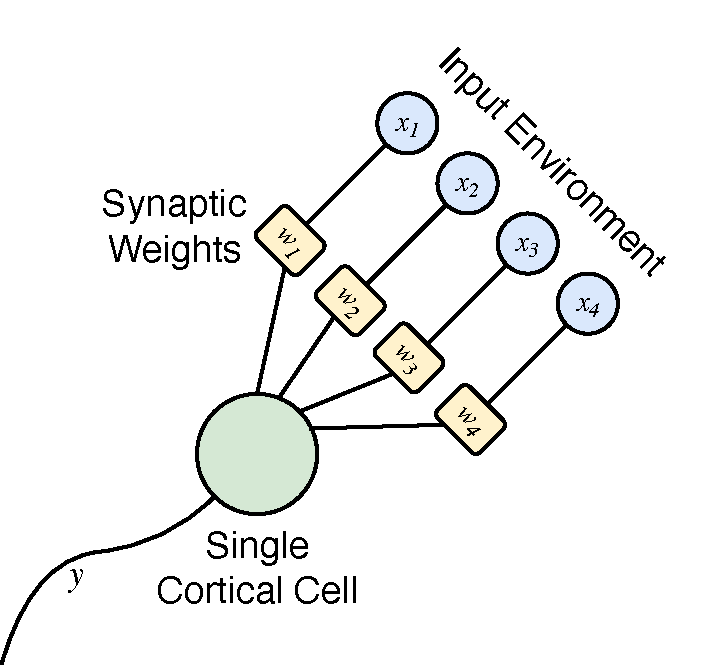
\includegraphics{/Users/bblais/Documents/Git/Amblyopia-Simulation/Manuscript/resources/Simple Neuron.pdf}
\caption{Simple model of a neuron with 4 inputs (\(x_1, x_2, x_3,\) and
\(x_4\)), connecting to the cell via 4 synaptic weights
(\(w_1, w_2, w_3,\) and \(w_4\)), yielding an output
(\(y\)).}\label{fig:simple_neuron}
\end{figure}

\subsection{Plasticity}\label{sec:plasticity}

The BCM theory states that the synaptic weights change depending on the
input to those weights, the output of the neuron, and a sliding
threshold according to the following equations,
\begin{equation}\phantomsection\label{eq:bcm1}{
\frac{dw_i}{dt} = \eta y(y-\theta_M) x_i
}\end{equation}

\begin{equation}\phantomsection\label{eq:bcm2}{
\frac{d\theta_M}{dt} = (y^2-\theta_M)/\tau
}\end{equation}

where is \(x_i\) is the \(i\)th presynaptic input, \(w_i\) is the
\(i\)th synaptic weight, and \(y\) is the postsynaptic output activity.
In Equation \ref{eq:bcm1}, the weights increase if the output, \(y\), is
above the threshold, \(\theta_M\), and decrease if the output is below
the threshold. The sliding threshold, \(\theta_M\), follows postsynaptic
activity in a non-linear way (Equation \ref{eq:bcm2}) and serves to
stabilize any runaway weights and the combination of the two equations
enforces the selectivity property of the BCM neuron\textsuperscript{2}.
The constant, \(\eta\), refers to the learning rate and the constant,
\(\tau\), is what we call the memory constant and is related to the
speed of the sliding threshold. These parameters influence the overall
rate of synaptic plasticity and are generally held constant for any
series of simulations so that relative dynamics can be compared.

The form of the BCM equations is what is called the \emph{quadratic
form} and represents the simplest way of writing the minimum
requirements of the BCM theory, but other forms have also been
explored\textsuperscript{3,4}.

\begin{figure}
\centering
\includesvg{/Users/bblais/Documents/Git/Amblyopia-Simulation/Manuscript/resources/fig-bcm-phi.svg}
\caption{The BCM synaptic modification function. Units are
arbitrary.}\label{fig:fig-bcm-phi.svg}
\end{figure}

\subsection{Selectivity}\label{sec:selectivity}

One of the properties of the BCM learning rule is that in most
environments the neuron becomes \emph{selective} -- it responds to a
small subset of the environment and has low or zero responses to the
rest of the environment. We can see this by looking at the response of
the neuron, \(y\), across the entire environment. Imagine that there are
two possible patterns:

\begin{enumerate}
\def\labelenumi{\arabic{enumi}.}
\tightlist
\item
  input \#1 is \emph{strongly} active and input \#2 is weakly active
\item
  input \#2 is \emph{strongly} active and input \#1 is weakly active
\end{enumerate}

At the start, the BCM neuron responds strongly to both patterns about
the same amount of time. After learning, the BCM becomes selective -- it
responds to only one of the patterns strongly most of the time, and the
other pattern yields a weak response as shown in Figure
\ref{fig:output_dist_2d}. This distribution is \emph{bimodal} -- there
is a cluster of responses above zero and one below zero, separated by a
gap of no responses. When we think of selective responses we often think
in terms of bimodal output distributions. We will see later that this is
not a general property of selective responses, however it is an
intuitive way of thinking about them.

\begin{figure}
\centering
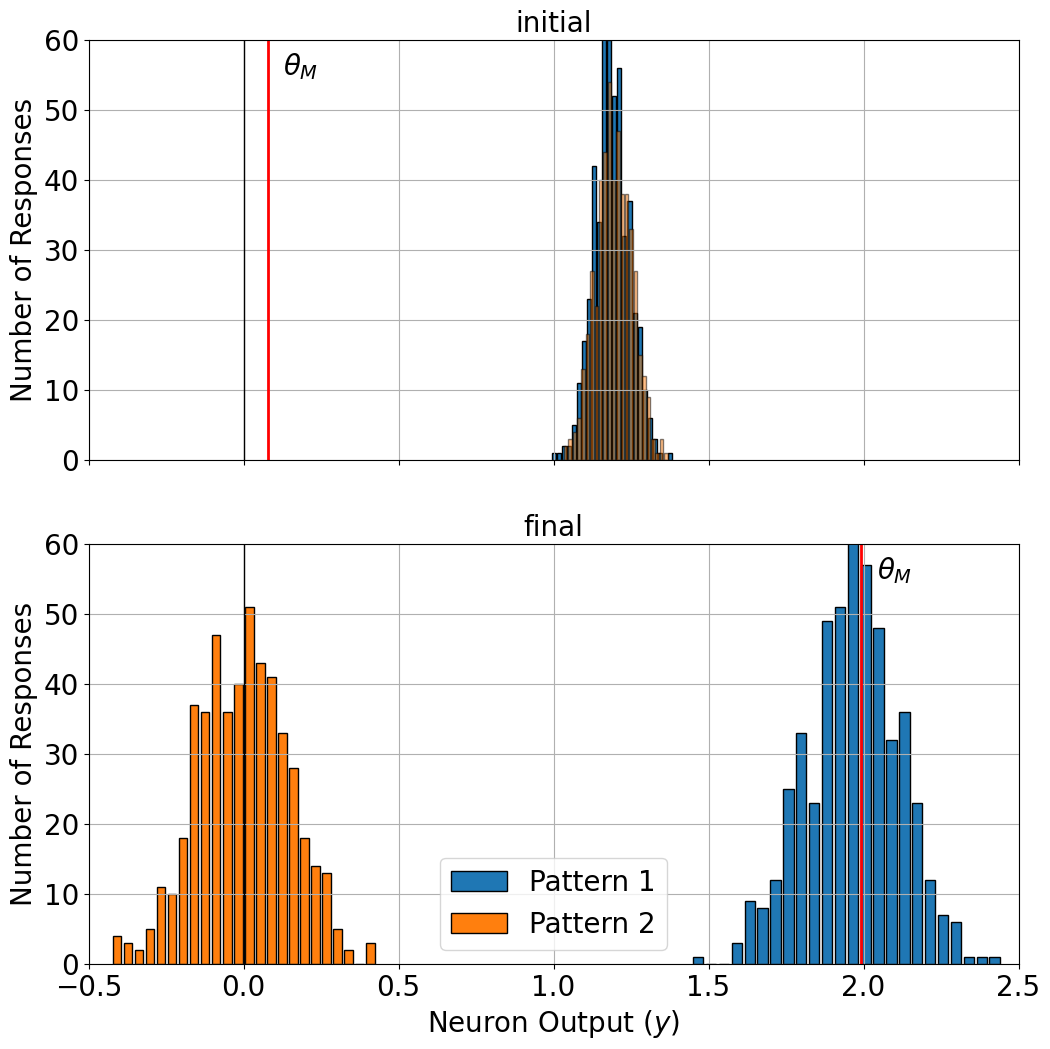
\includegraphics{/Users/bblais/Documents/Git/Amblyopia-Simulation/Manuscript/resources/Pasted image 20240123131156.png}
\caption{The output distribution for a BCM neuron. The initial
distribution (above) shows that the BCM neuron responds strongly to both
patterns about the same amount of time. The final distribution (below)
shows that the BCM neuron responds to only one of the patterns strongly
most of the time, and the other pattern yields a weak response. This
distribution is \emph{bimodal} -- there is a cluster of responses above
zero and one below zero, separated by a gap of no responses. Also notice
that the modification threshold, \(\theta_M\), settles on the value of
the neural output for the selected pattern.}\label{fig:output_dist_2d}
\end{figure}

Geometrically we can plot the input patterns by plotting the activity of
input \#1 on the x-axis and the activity of input \#2 on the y-axis --
this shows 2 primary clusters, as shown in Figure \ref{fig:2d_inputs}.

We can also show the values of the weights as a ``dot'' on this plot,
with the weight for input \#1 on the x-axis and the weight for input \#2
on the y-axis. Visually, it is easier to see it by drawing a line from
the origin to this dot. The output distribution is formed by projecting
a perpendicular from the inputs to this line, as shown in Figure
\ref{fig:2d_initial_weights_outputs} for the initial weights and Figure
\ref{fig:2d_final_weights_outputs} for the final weights. Geometrically,
for the weights to have weak responses to an input pattern then the
weights must be \emph{perpendicular to that input pattern}. One can see
this for the final weights and pattern \#2 in these figures.

\begin{figure}
\centering
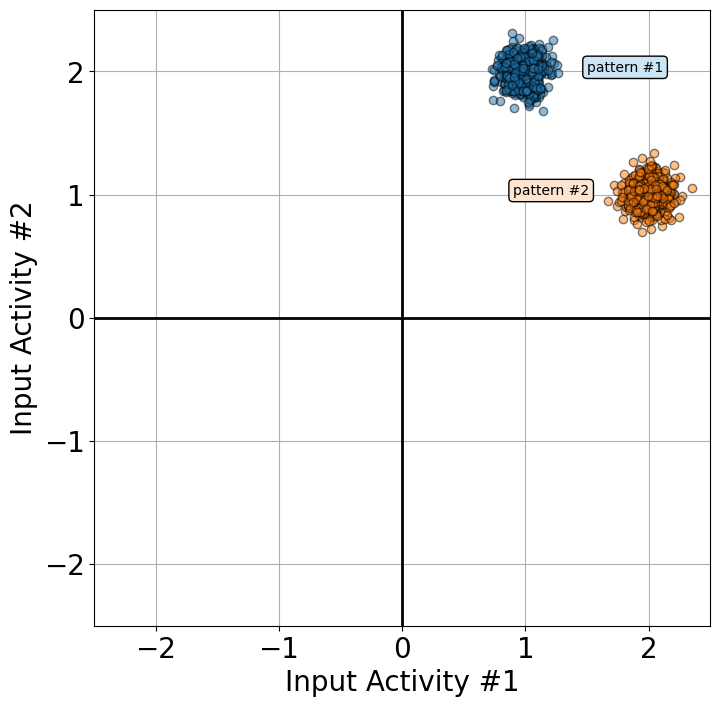
\includegraphics{/Users/bblais/Documents/Git/Amblyopia-Simulation/Manuscript/resources/Pasted image 20240123130523.png}
\caption{2D input environment. .}\label{fig:2d_inputs}
\end{figure}

\begin{figure}
\centering
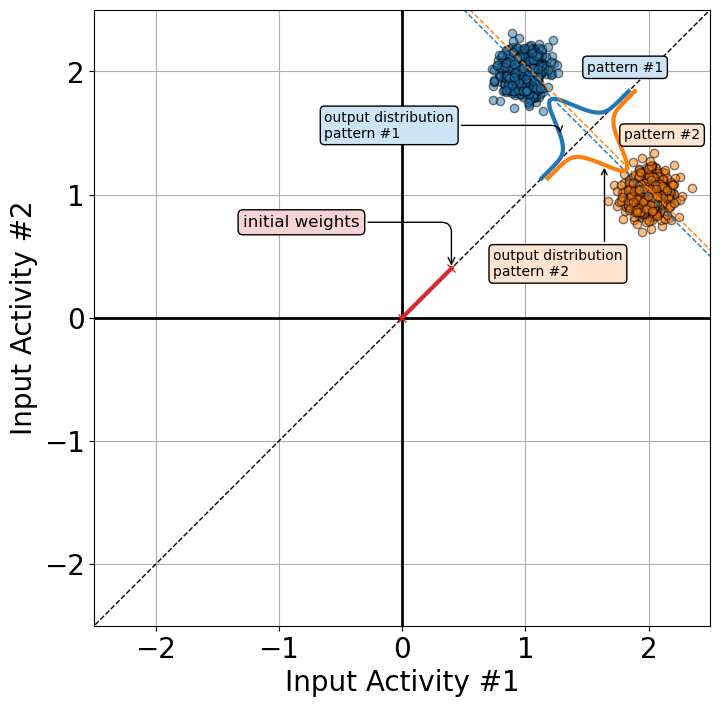
\includegraphics{/Users/bblais/Documents/Git/Amblyopia-Simulation/Manuscript/resources/Pasted image 20240123130539.png}
\caption{Geometric interpretation of the weights and output
distributions for the \emph{initial weights} in a 2D input environment.
.}\label{fig:2d_initial_weights_outputs}
\end{figure}

\begin{figure}
\centering
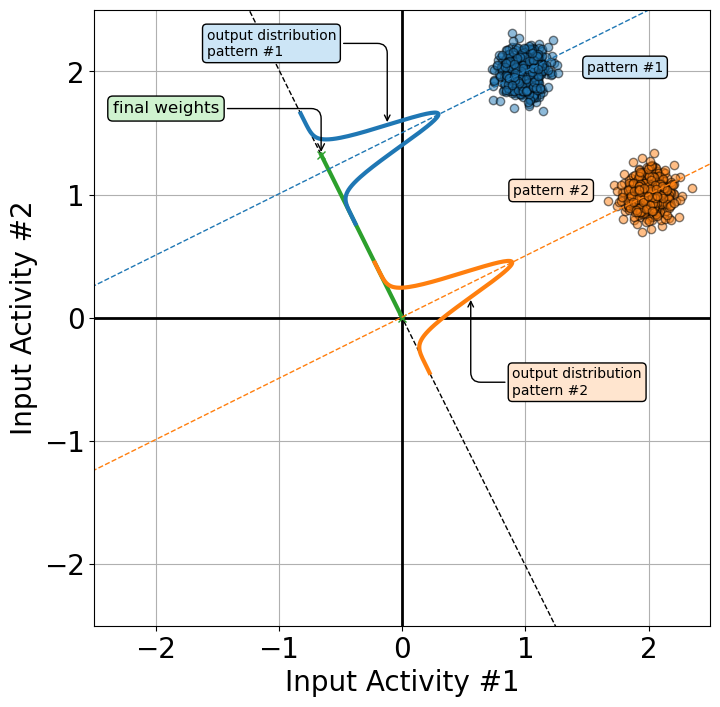
\includegraphics{/Users/bblais/Documents/Git/Amblyopia-Simulation/Manuscript/resources/Pasted image 20240123130559.png}
\caption{Geometric interpretation of the weights and output
distributions for the \emph{final weights} in a 2D input
environment.}\label{fig:2d_final_weights_outputs}
\end{figure}

\subsection{Natural Images}\label{sec:natural-images}

\begin{figure}
\centering
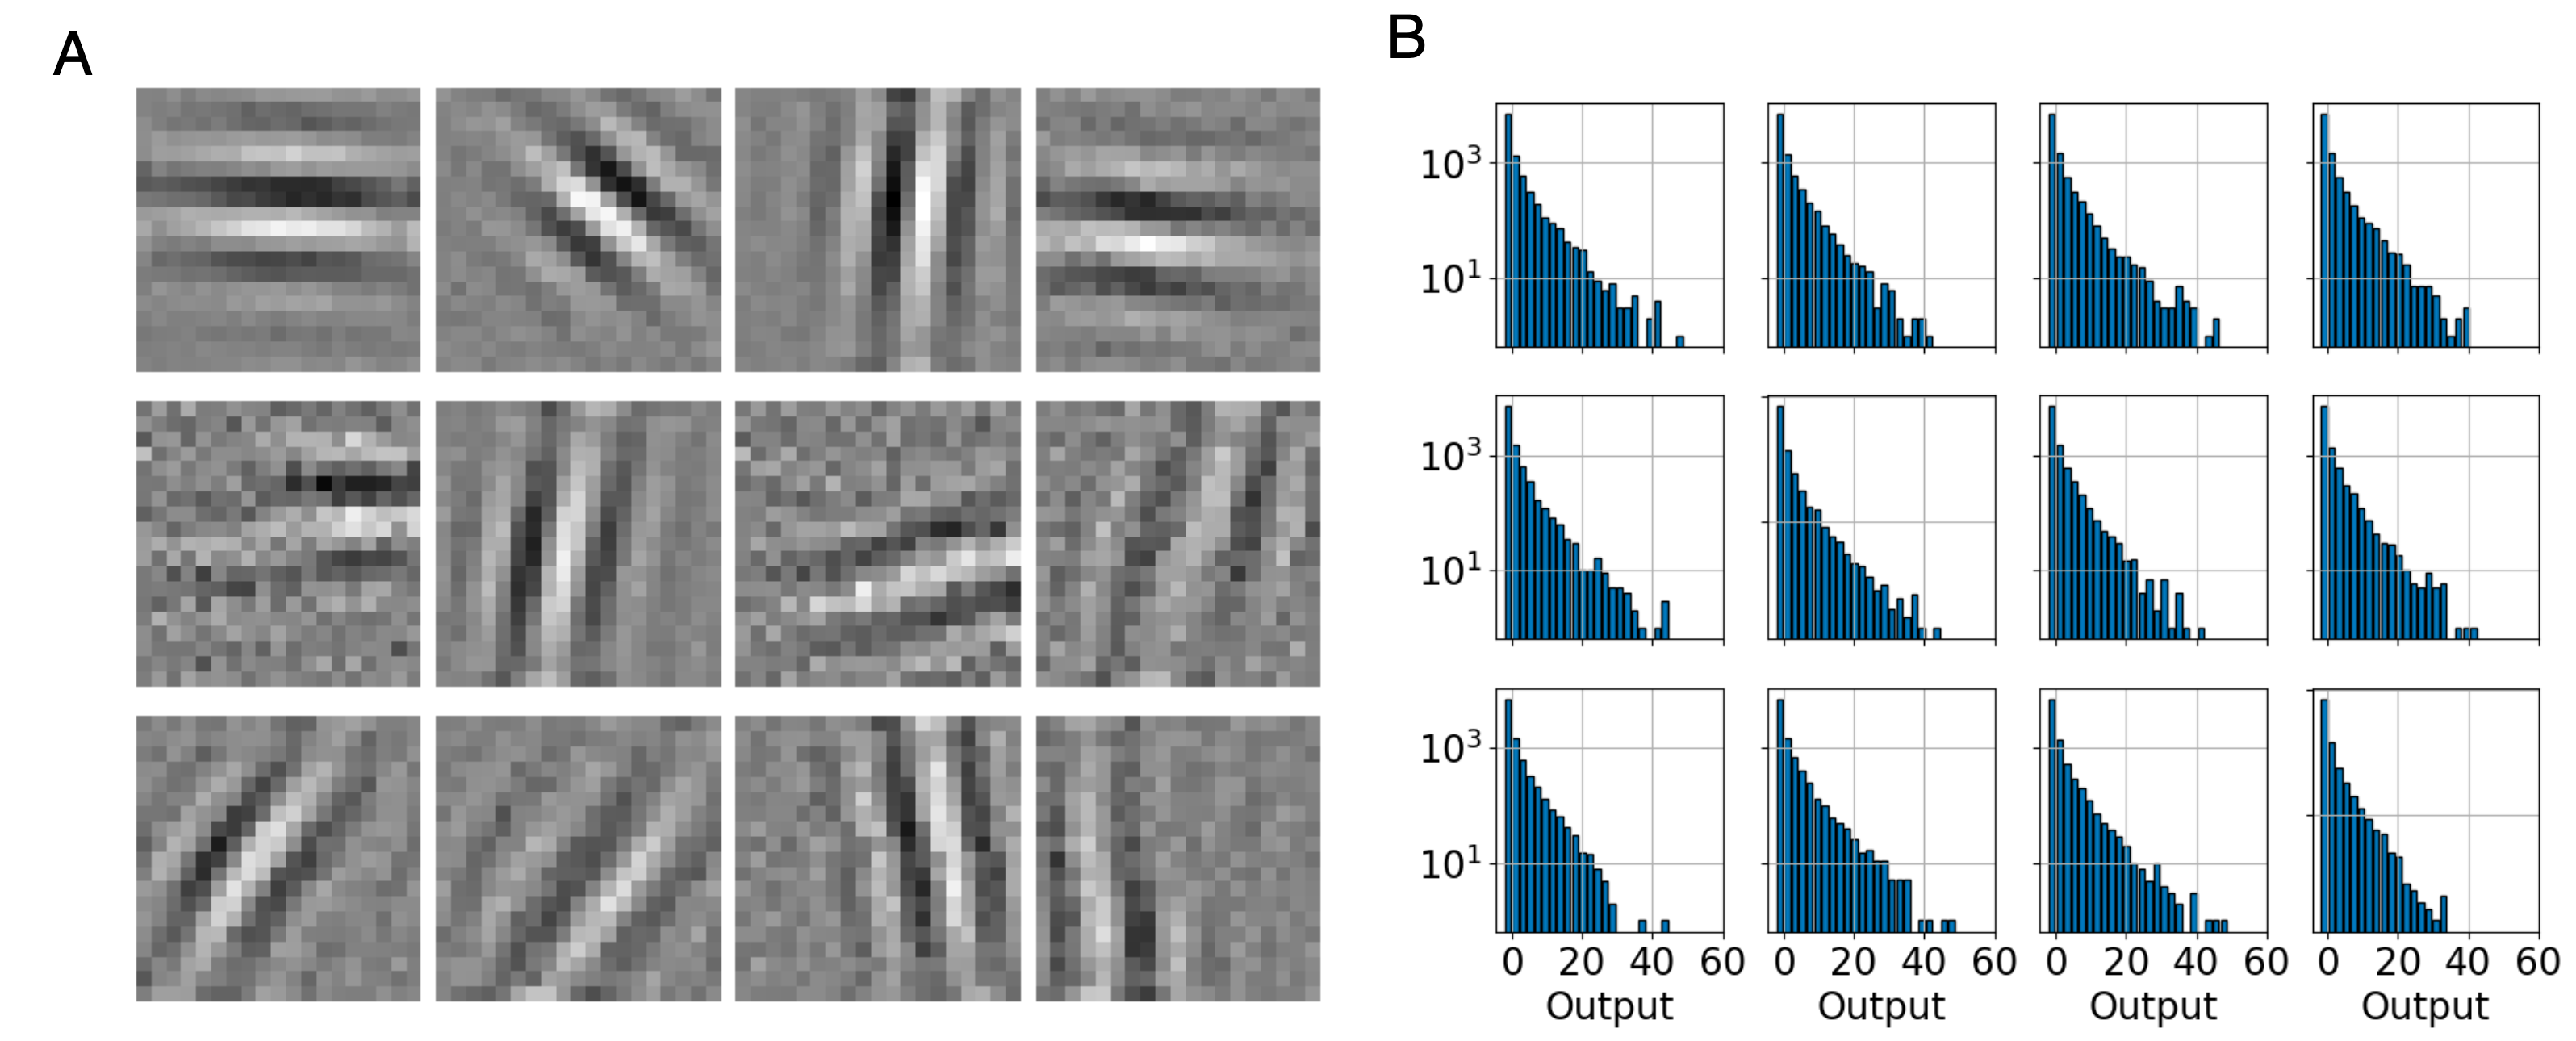
\includegraphics{/Users/bblais/Documents/Git/Amblyopia-Simulation/Manuscript/resources/weights and output distribution natural images.drawio.png}
\caption{Weights (A) and Output distributions (B) for 12 neurons trained
with natural image input patterns. The weights are shown in grayscale,
with black representing low weights and white representing high weights.
The output distribution is shown on a log scale to highlight the few
patterns that yield the strongest
responses.}\label{fig:nat_image_weights_and_output_dist}
\end{figure}

Shown in Figure \ref{fig:nat_image_weights_and_output_dist} are the
weights and output distributions for 12 neurons trained with natural
image input patterns. We easily see that the neurons are selective to
orientation -- the final weights are organized in a line at a particular
orientation. Thus, any input pattern that has that same orientation will
elicit stronger responses because the pattern will align with the strong
weights. Unlike the low dimensional case earlier, the output
distributions for each neuron is \emph{not bimodal}. The output
distribution does not show a cluster above zero and a cluster at zero
with a gap in between, it is smeared out over the entire range of the
responses. What makes the neuron selective is the fact that the vast
bulk of the responses are near zero, and while there is no gap between
low and high responses, the number of patterns yielding strong responses
is very small. Note that the output distributions are being shown on a
log scale, otherwise those strong responses would not even be visible.

This observation means that what BCM neurons select in an environment is
not always \emph{clusters} but a small number of patterns in a sea of
similar patterns. Statistically, this means that BCM is sensitive to
statistics in the input environment beyond separability and 2-point
correlations\textsuperscript{5}. In order to understand the dynamics of
BCM neurons we can explore environments with patterns that don't fall
into neat clusters but instead are spread out with higher order
statistics.

\subsection{Structure vs Noise}\label{sec:structure-vs-noise}

The basic intuition behind the dynamics of the neuron, as it experiences
the changing input environment, comes from an understanding of the
competition between \emph{structure} and \emph{noise}. These terms refer
to the statistics of the input environment and the mathematical form of
the plasticity equations -- different sets of equations will respond to
different forms of \emph{structure} and have different dynamics under
\emph{noise}. This can be used to compare different theories of synaptic
plasticity\textsuperscript{6} but is beyond what we want to discuss
here.

In the case of the BCM theory, the \emph{structure} comes in the form of
an environment with a minority of patterns yielding high responses and
the majority yielding low responses -- the BCM neuron can become
selective in this environment. \emph{Noise} by definition does not have
this property. It is either random variation on top of the structure or
random input without the patterns that can lead to high responses.
Gaussian (i.e.~normal) noise is an example of such variation. Examples
of structure and noise can be visually seen in Figure
\ref{fig:structure_vs_noise}.

\begin{figure}
\centering
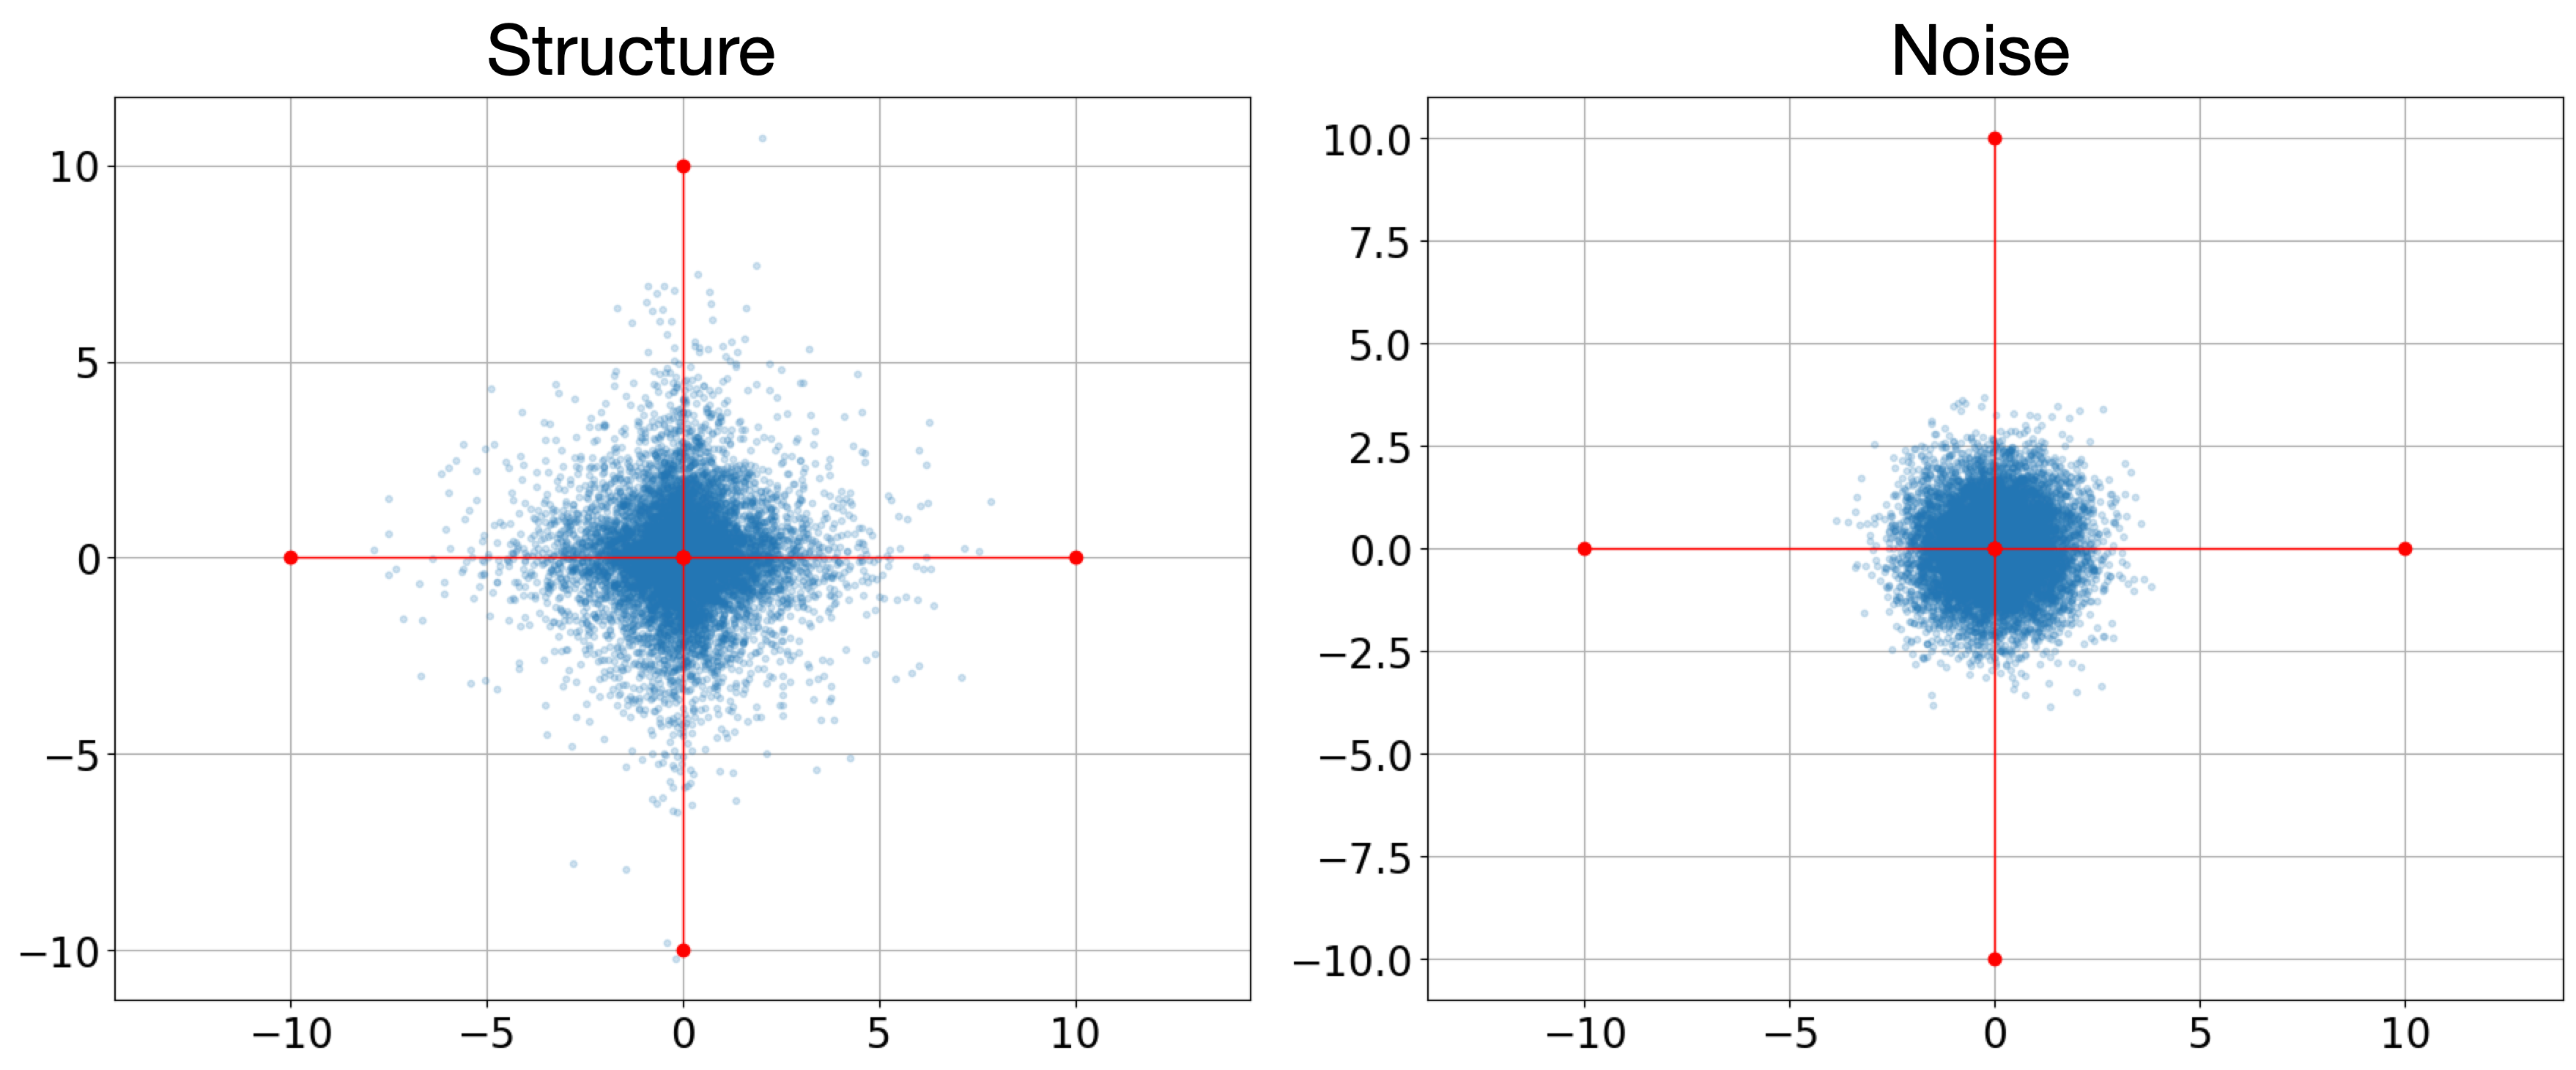
\includegraphics{/Users/bblais/Documents/Git/Amblyopia-Simulation/Manuscript/resources/Pasted image 20240117155651.png}
\caption{Structure (left) and noise (right) for a BCM neuron. Shown on
the axes are the input values for a two-input neuron, the value of input
\(x_1\) shown on the x-axis and input \(x_2\) on the y-axis. Each tiny
blue dot is a snapshot of the activity of \((x_1,x_2)\) at some time.
Over time, as the neuron experiences the environment, the activity plot
fills in the cloud shown. In the case of structure can see a minority
input values that are high, extending out in the x- and y-directions
compared to the noise (right figure) where all directions are equal. In
the structured environment, the weights for the BCM neuron converge to
those directions such that the postsynaptic response is
selective.}\label{fig:structure_vs_noise}
\end{figure}

The \emph{structure} in this case is generated using a distribution
known as the Laplace distribution, or double exponential \[
P(x) \sim e^{-|x|}
\]

The \emph{noise} is generated using a Gaussian or Normal distribution,
\[
P(x) \sim e^{-x^2}
\] Mathematically the difference leads to the Laplace environment having
more values near zero and a significant number of patterns at very high
values (compared to the Gaussian) -- rare patterns. This property of the
Laplace distribution (and some other distributions) is sometimes
referred to as having ``heavy tails''. This mathematical property is
exactly the property the BCM neuron selects for when it learns, so we
expect the BCM to become selective in an environment produced by a
Laplace distribution vs a Gaussian one. We can see the property of rare
input patterns by looking at the distribution itself as in Figure @
\ref{fig:laplace_dist}, shown on a semi-log plot do highlight those
high-value patterns. Compared to a Gaussian, the Laplace distribution
has many more patterns with significantly higher values. The natural
image environment also has a similar structure to the Laplace
environment, even for individual pixels as also shown in Figure @
\ref{fig:laplace_dist}.

\begin{figure}
\centering
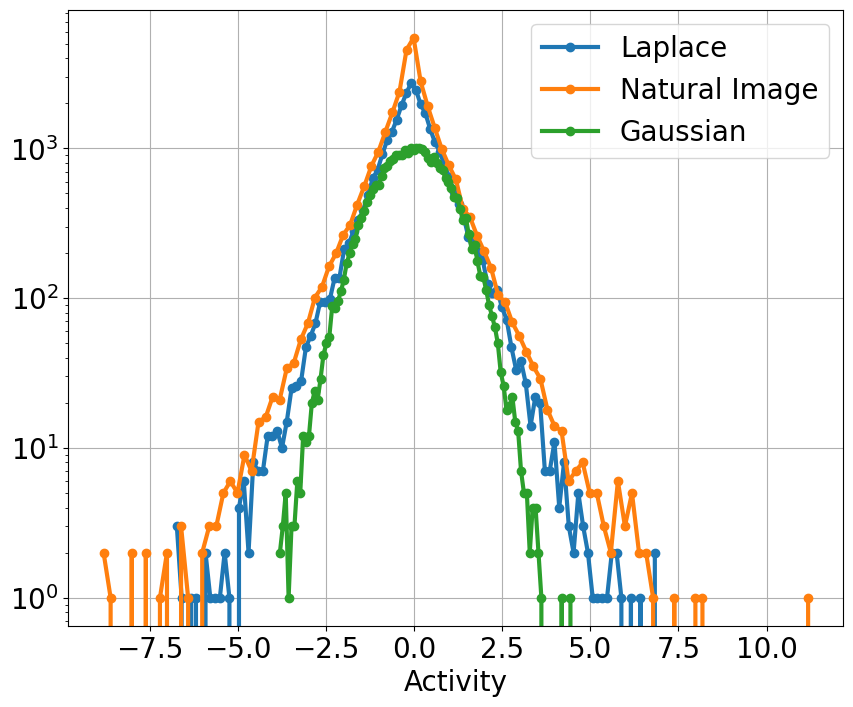
\includegraphics{/Users/bblais/Documents/Git/Amblyopia-Simulation/Manuscript/resources/Pasted image 20240228124006.png}
\caption{Single input (pixel) statistics for the Laplace environment and
the natural image environment compared to Gaussian (i.e.~Normal)
noise.}\label{fig:laplace_dist}
\end{figure}

As the BCM neuron learns, it starts with an output distribution more
similar to a Gaussian and learns to respond more to the rare patterns
with high activity, shown in Figure \ref{fig:2D_BCM_Laplace} for a 2D
Laplace environment and Figure \ref{fig:BCM_Natural_Image} for a natural
image environment. The rare patterns are the ones above the BCM
modification threshold, \(\theta_M\).

\begin{figure}
\centering
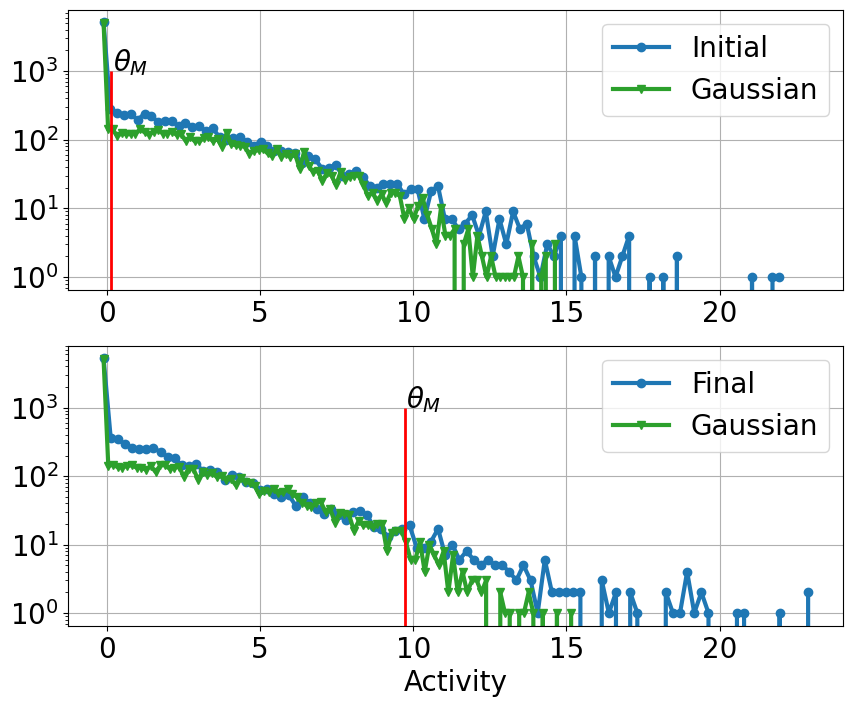
\includegraphics{/Users/bblais/Documents/Git/Amblyopia-Simulation/Manuscript/resources/Pasted image 20240228124702.png}
\caption{Output distributions for a BCM neuron in a 2D Laplace
environment. Shown are (top) the distribution of responses before any
learning and (bottom) after learning compared to a Gaussian distribution
of responses with the same standard deviation. In both cases, the
responses are smeared across the entire range, with fewer patterns
yielding high responses. Because these plots are on a log scale,
Gaussian responses appear curved down as activity increases while
Laplace responses appear as a straight decline. The BCM neuron finds
directions in the input space such that its responses are more Laplacian
-- they respond more to a smaller group of
patterns.}\label{fig:2D_BCM_Laplace}
\end{figure}

\begin{figure}
\centering
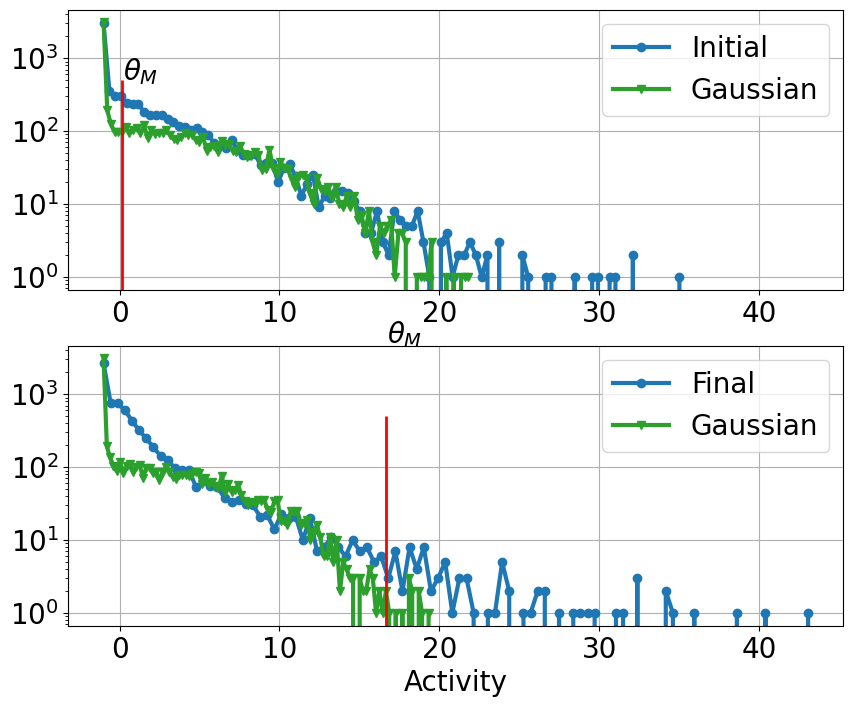
\includegraphics{/Users/bblais/Documents/Git/Amblyopia-Simulation/Manuscript/resources/Pasted image 20240228124932.png}
\caption{Output distributions for a BCM neuron in a natural image
environment. Shown are (top) the distribution of responses before any
learning and (bottom) after learning compared to a Gaussian distribution
of responses with the same standard deviation. In both cases, the
responses are smeared across the entire range, with fewer patterns
yielding high responses. Because these plots are on a log scale,
Gaussian responses appear curved down as activity increases while
Laplace responses appear as a straight decline. The BCM neuron finds
directions in the input space such that its responses are more Laplacian
-- they respond more to a smaller group of
patterns.}\label{fig:BCM_Natural_Image}
\end{figure}

\section{Normal and Deprived Visual
Environments}\label{sec:normal-and-deprived-visual-environments}

\begin{figure}
\centering
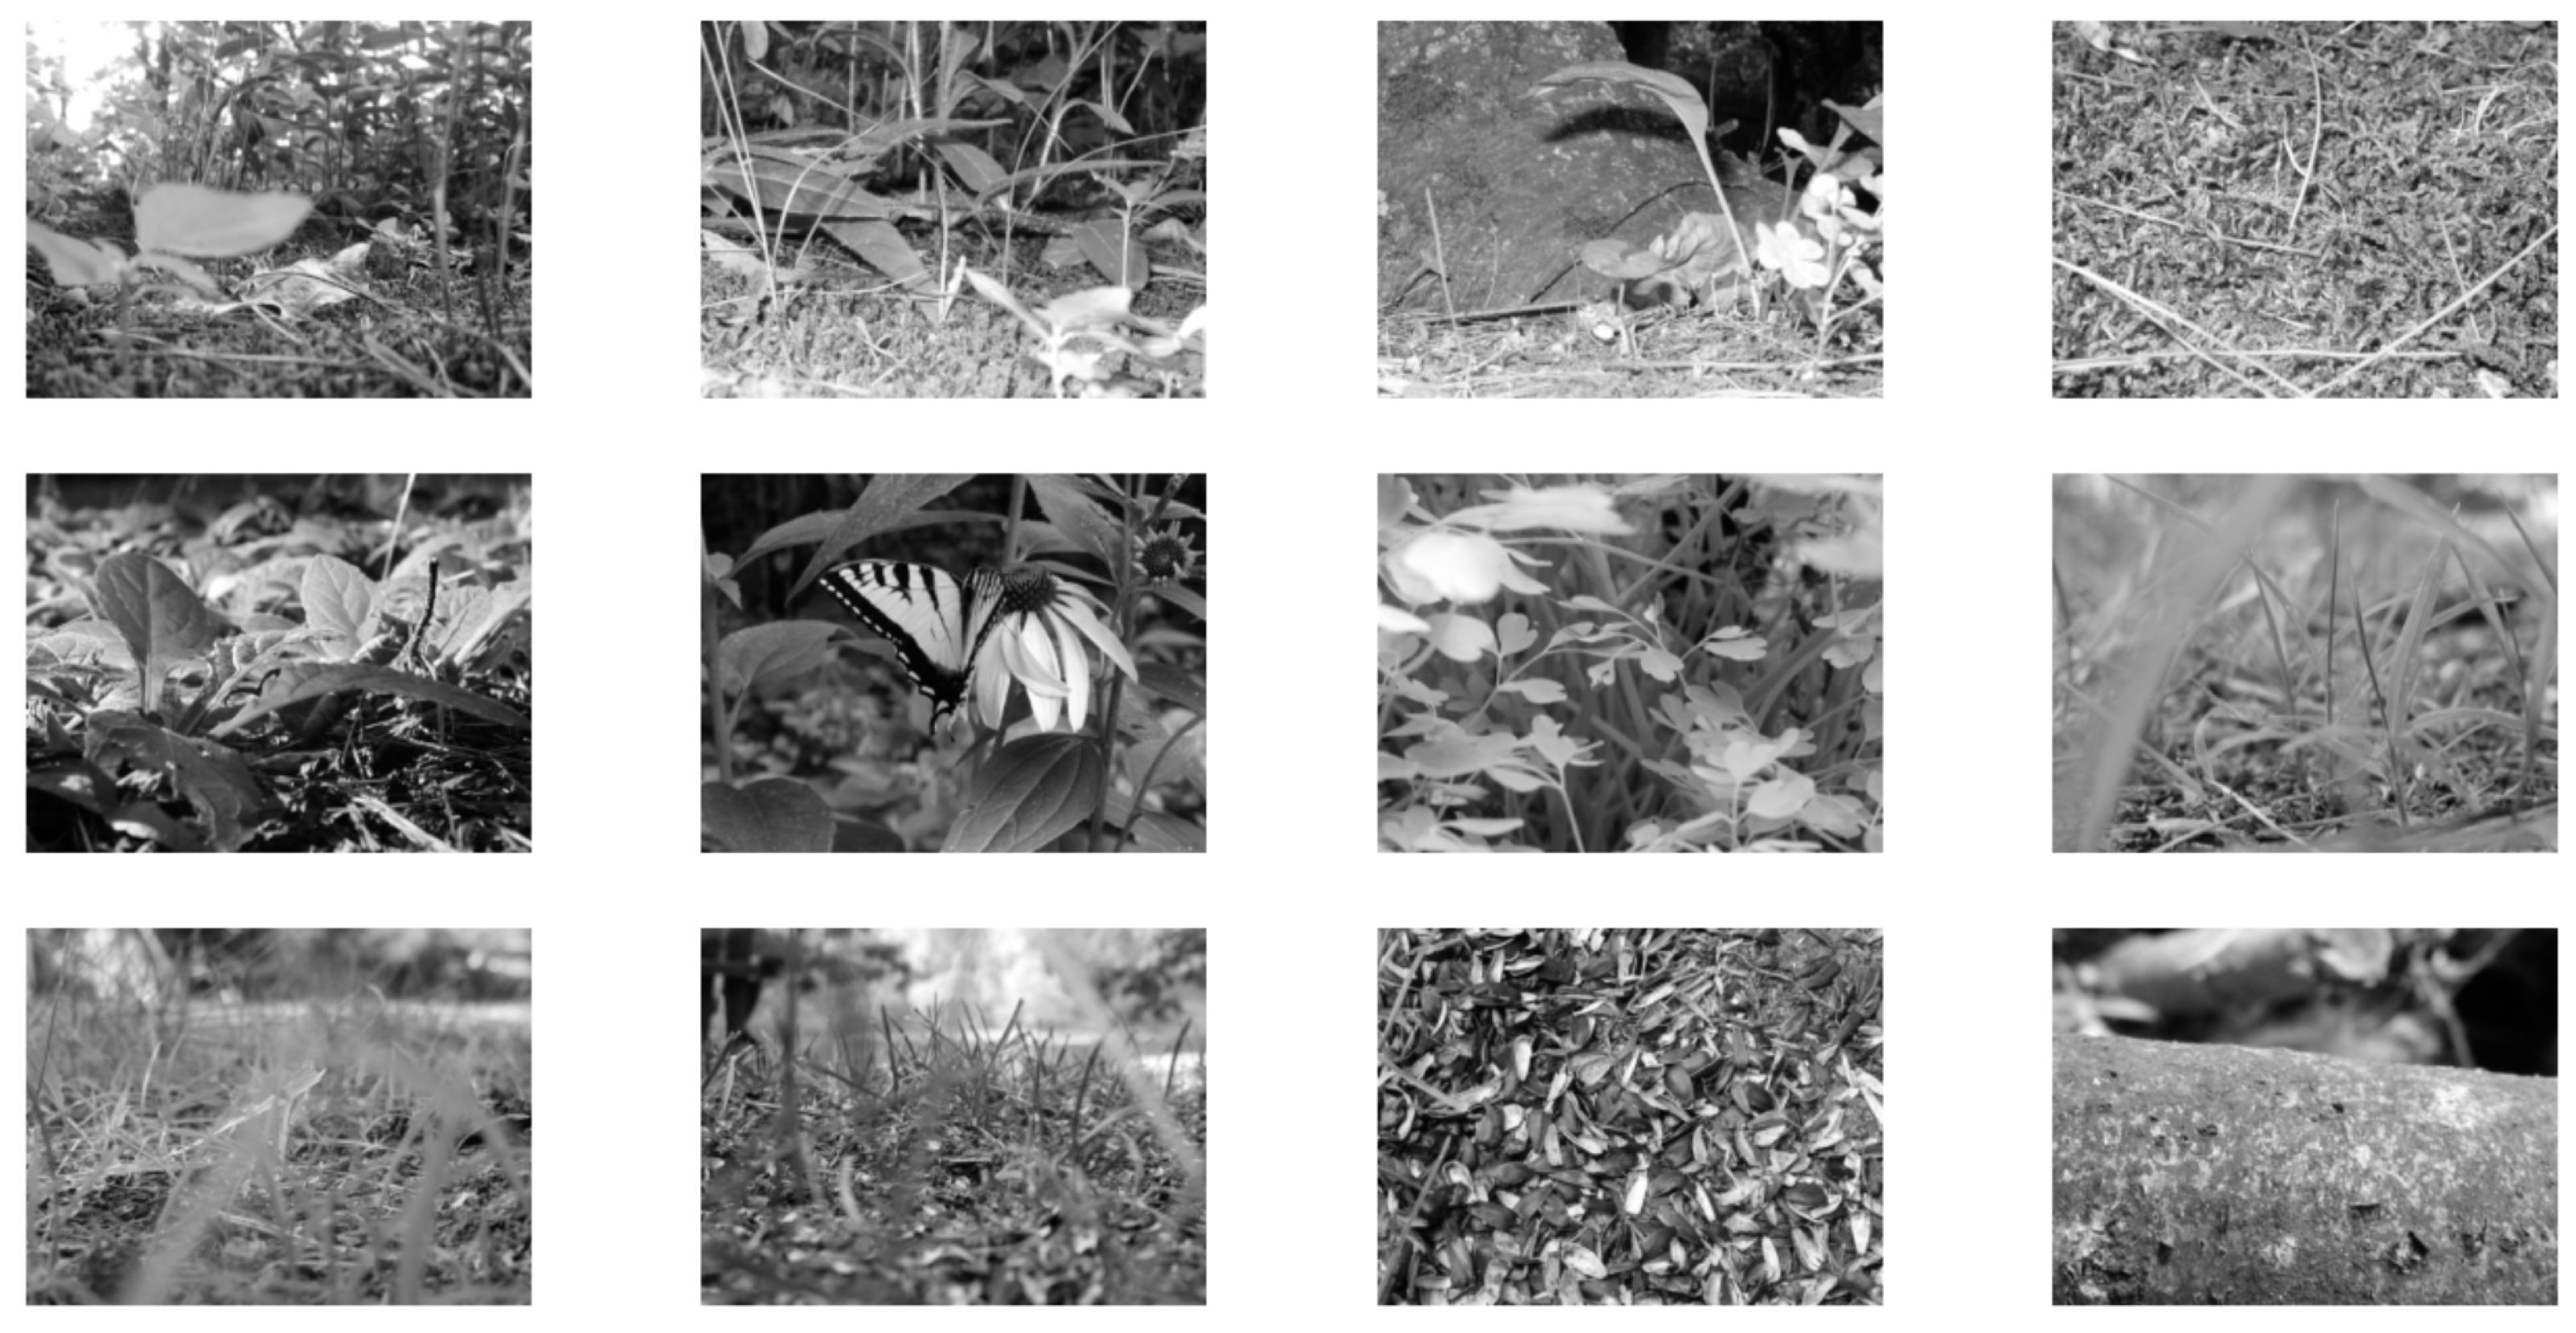
\includegraphics{/Users/bblais/Documents/Git/Amblyopia-Simulation/Manuscript/resources/Pasted image 20240301091111.png}
\caption{Natural Image Environment.}\label{fig:natural_images}
\end{figure}

\begin{figure}
\centering
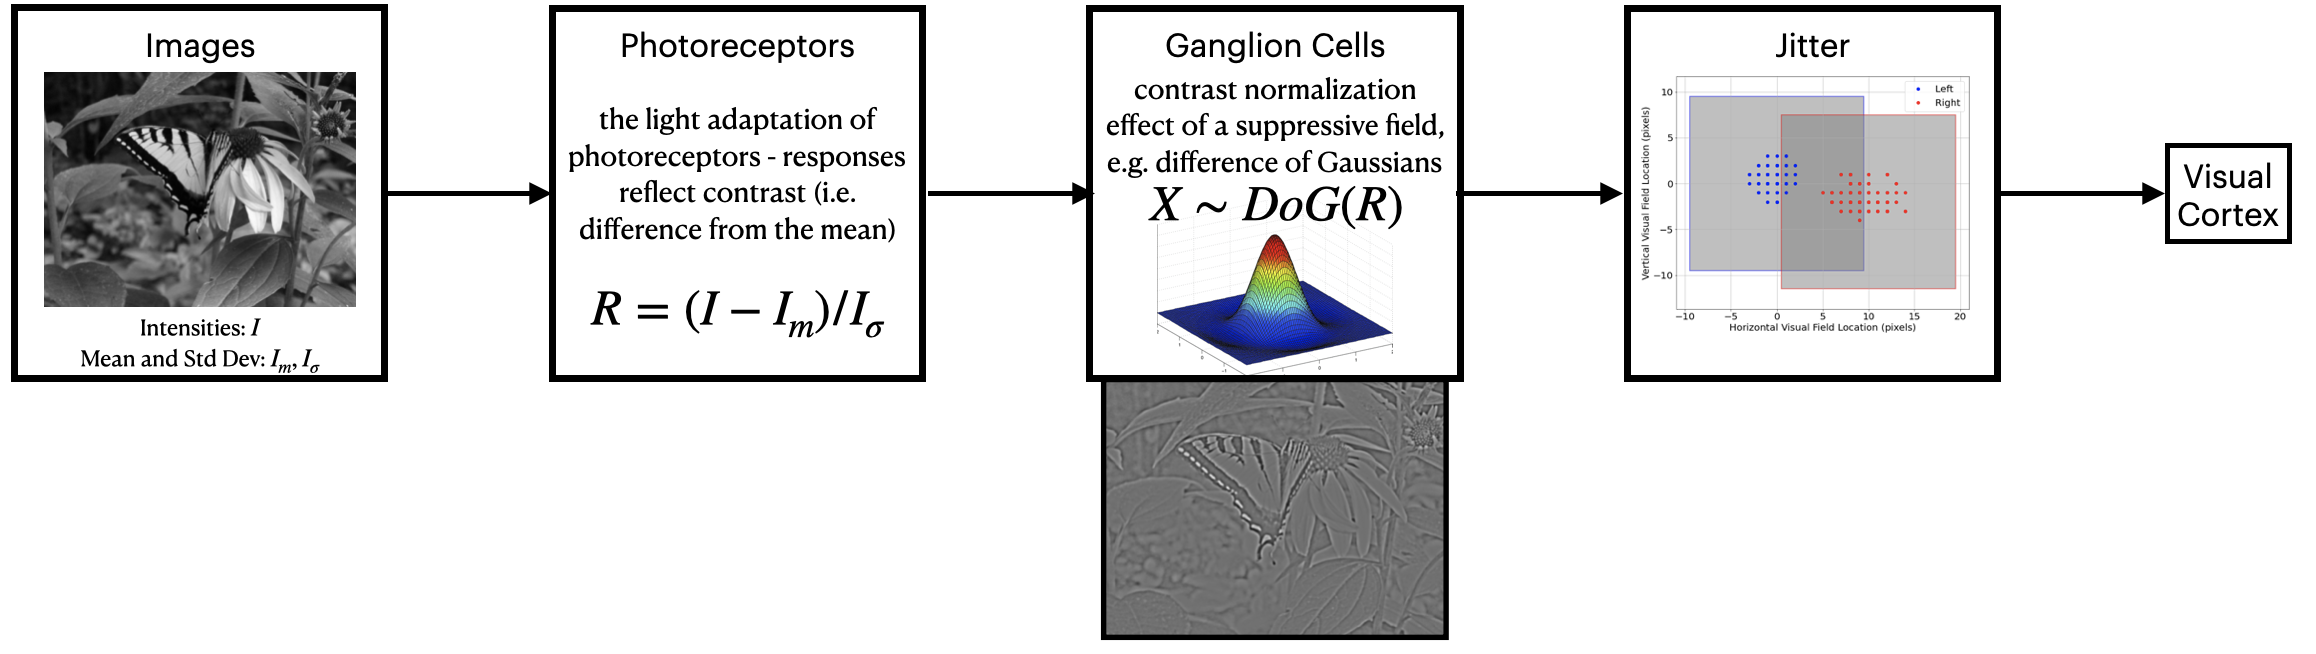
\includegraphics{/Users/bblais/Documents/Git/Amblyopia-Simulation/Manuscript/resources/Pasted image 20240301091213.png}
\caption{Normal Vision
Model.}\label{fig:Pasted_image_20240301091213.png}
\end{figure}

\begin{figure}
\centering
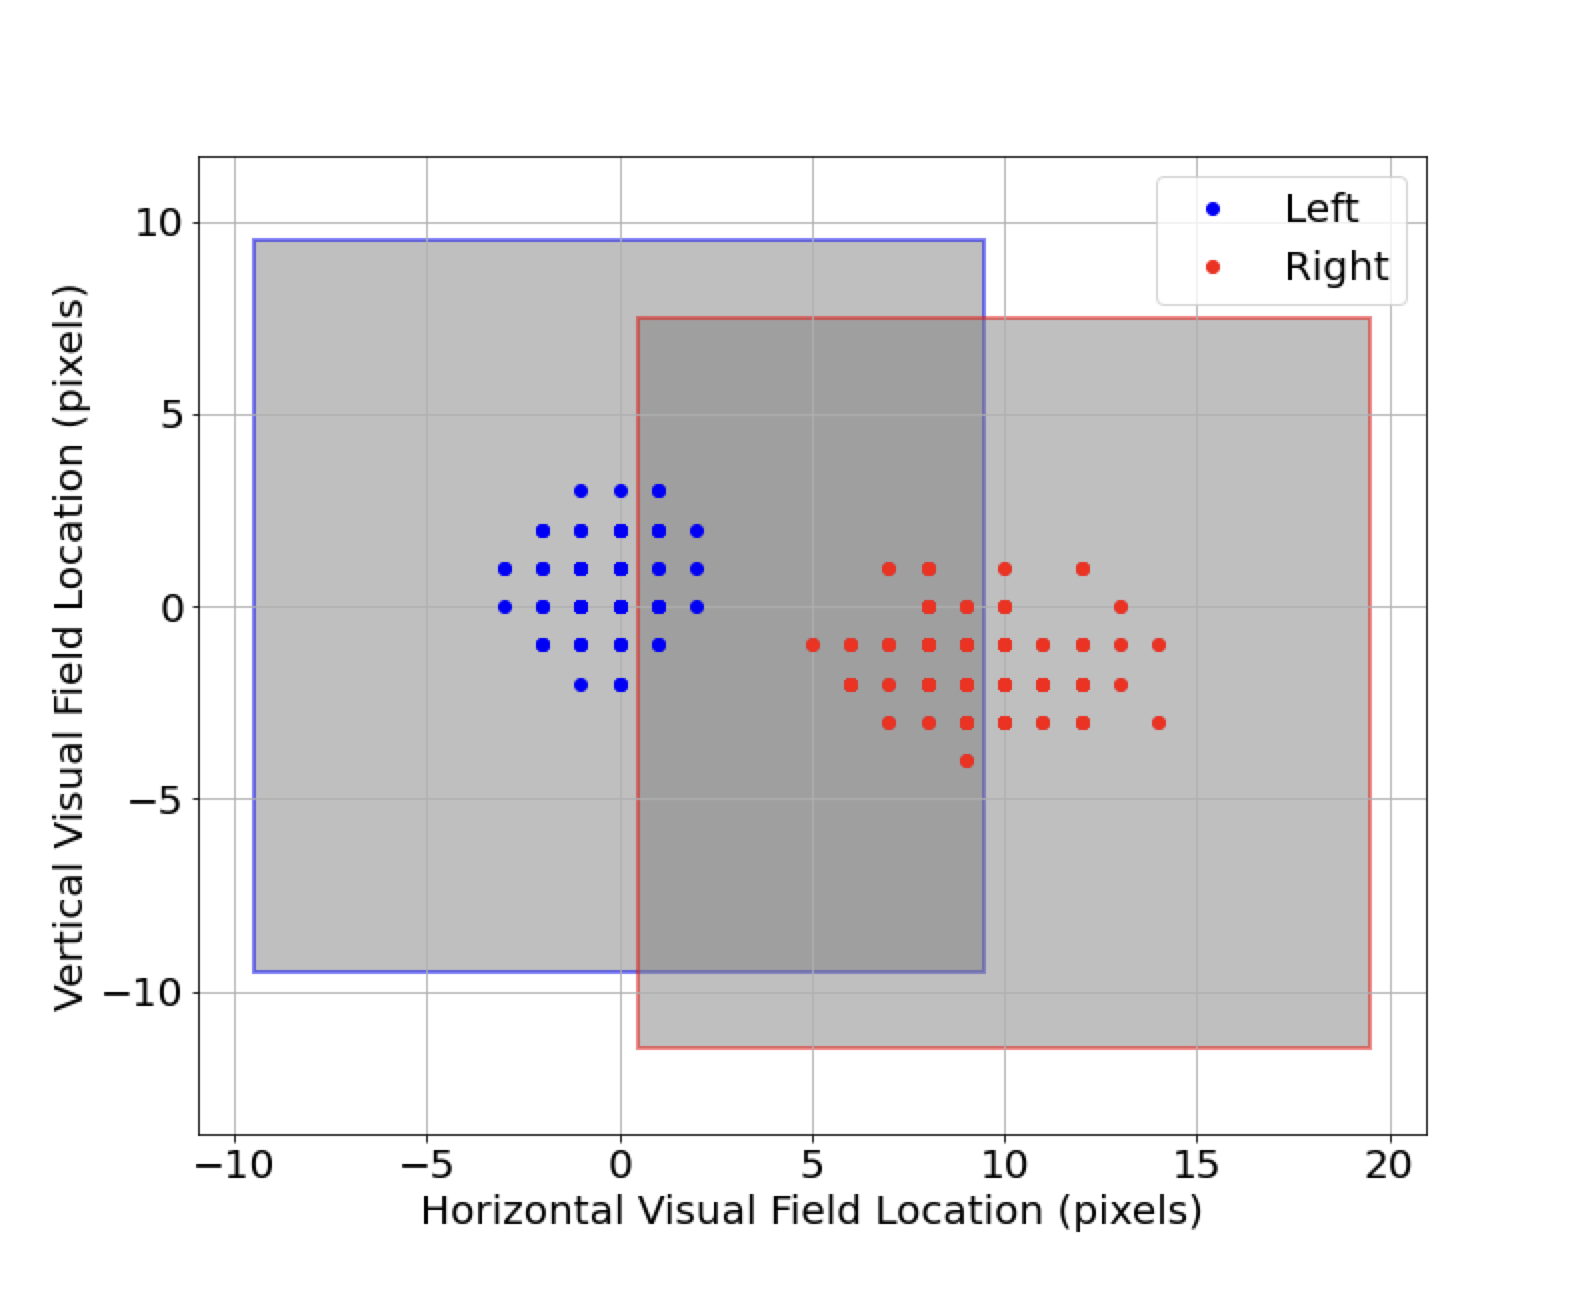
\includegraphics{/Users/bblais/Documents/Git/Amblyopia-Simulation/Manuscript/resources/Pasted image 20240301091231.png}
\caption{Model of Eye
Jitter.}\label{fig:Pasted_image_20240301091231.png}
\end{figure}

\begin{figure}
\centering
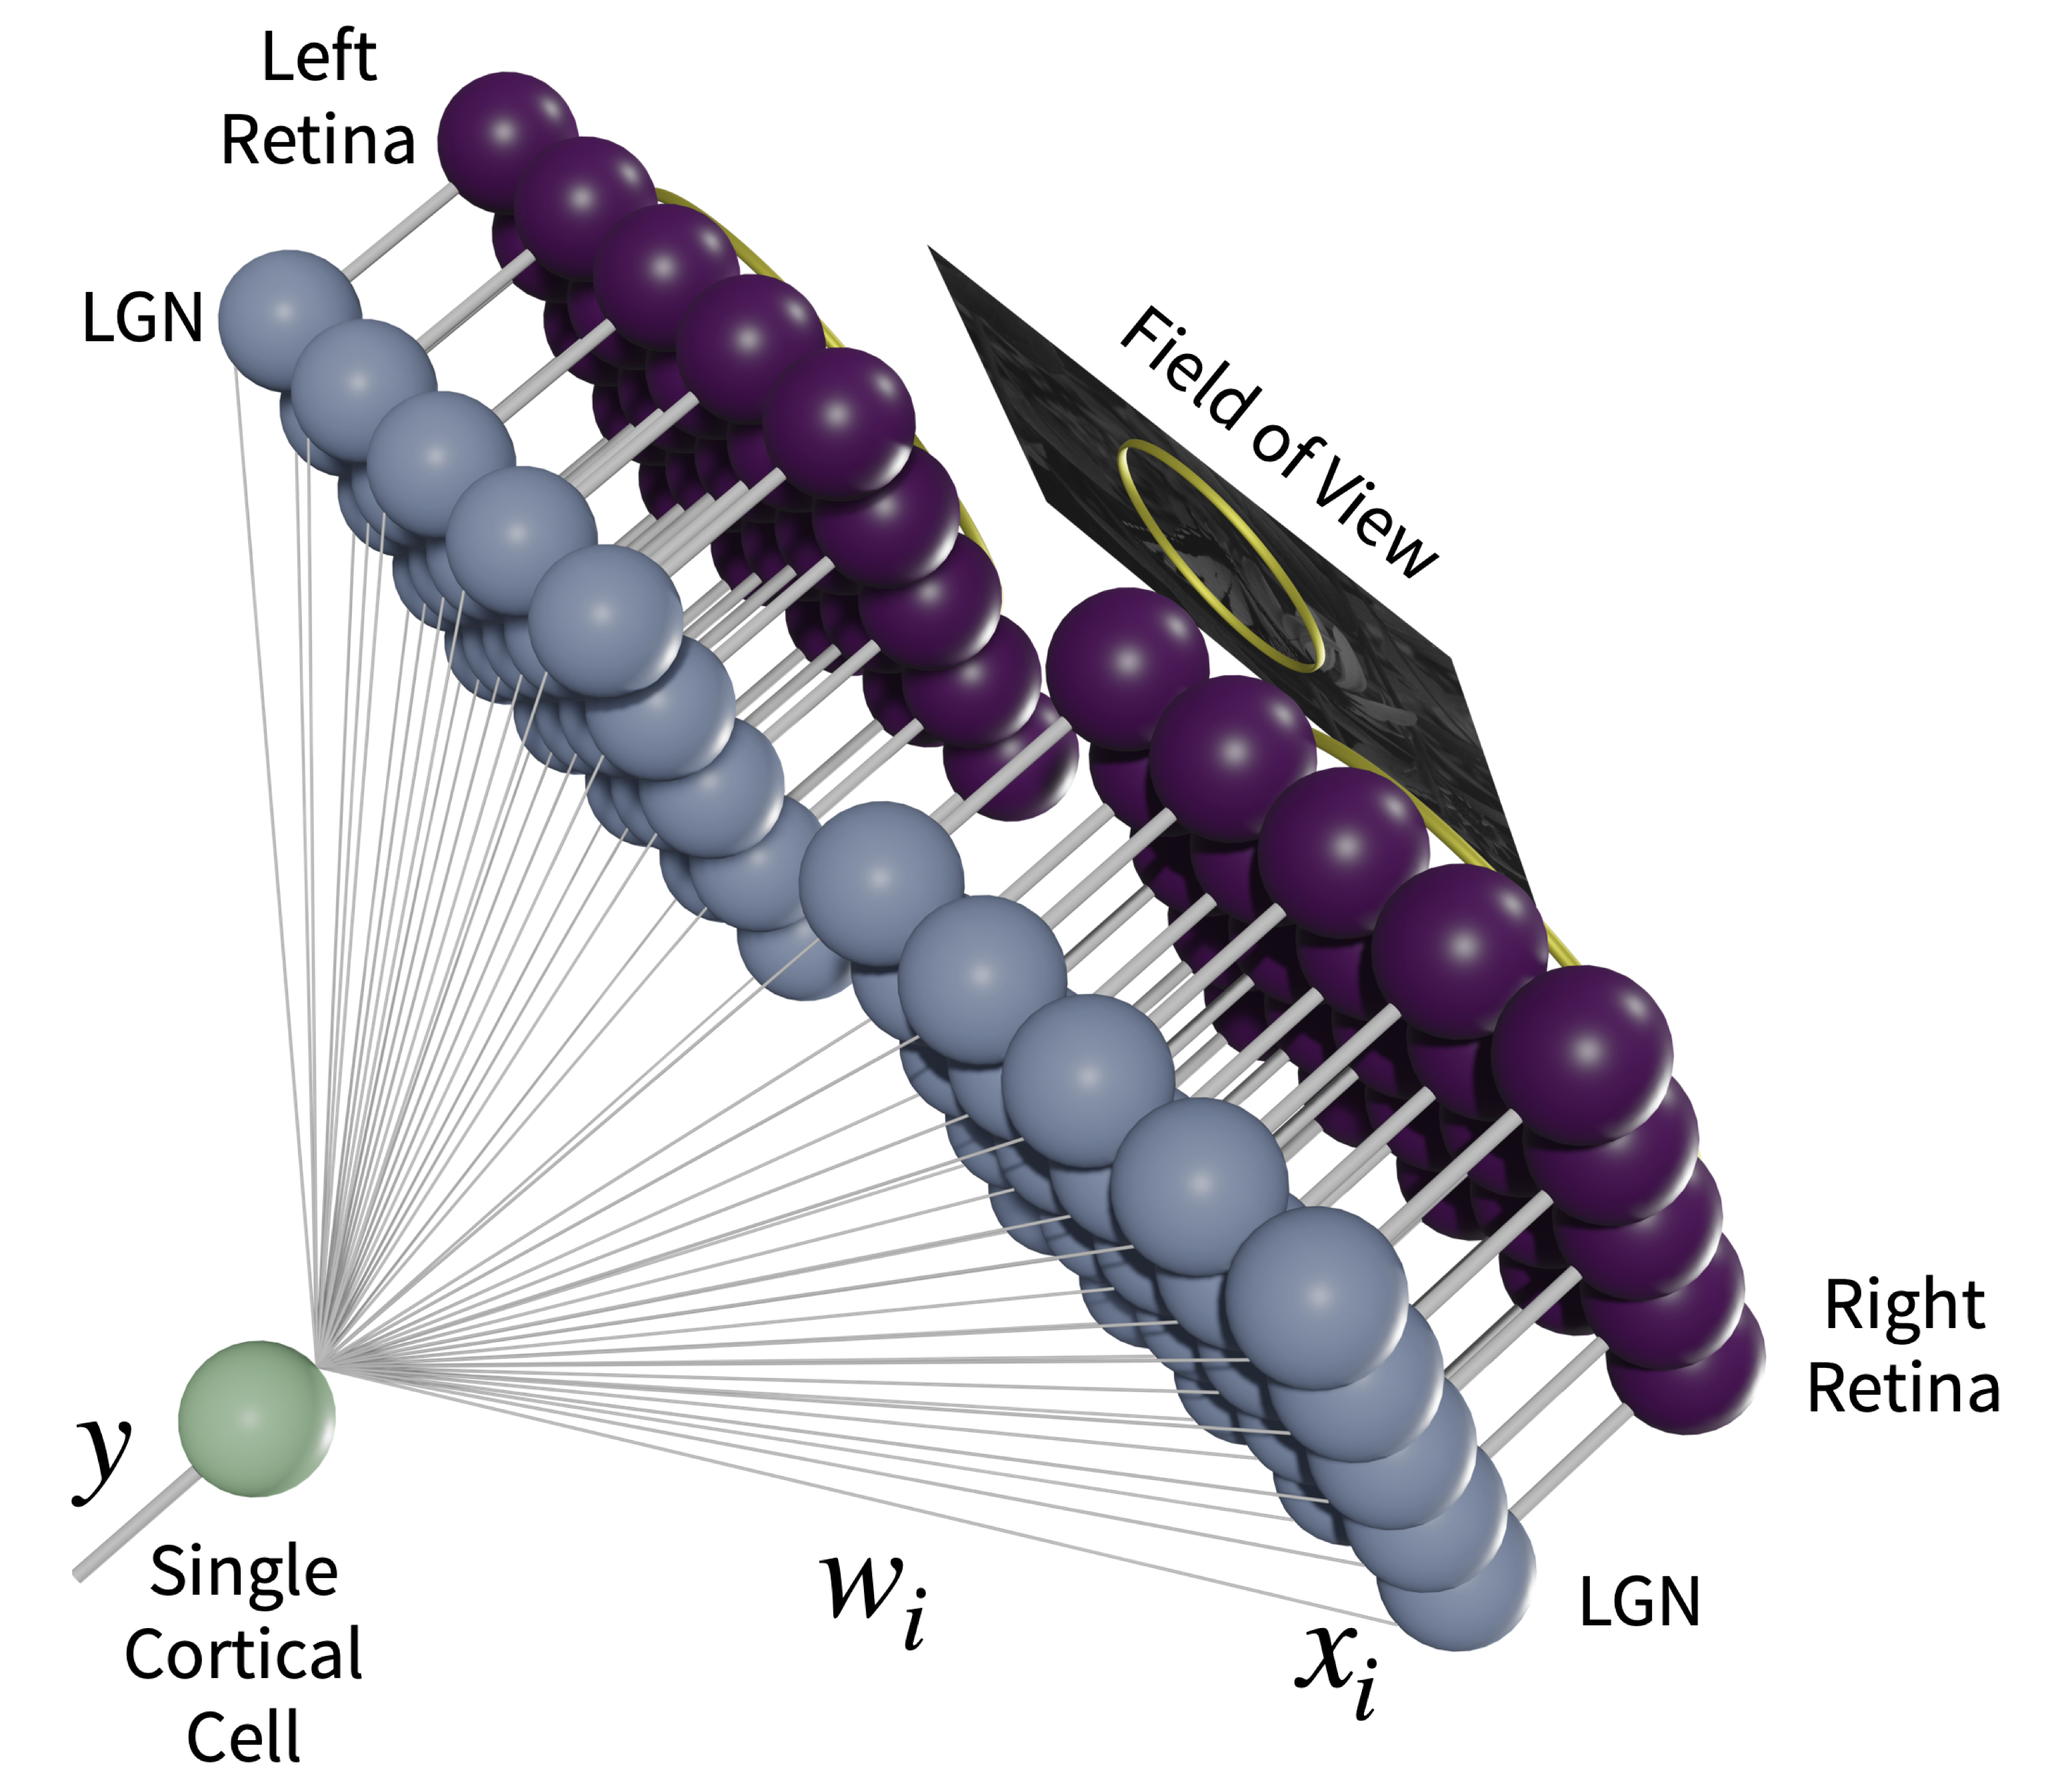
\includegraphics{/Users/bblais/Documents/Git/Amblyopia-Simulation/Manuscript/resources/Pasted image 20240301091247.png}
\caption{Architecture for binocular neurons in natural image
environment.}\label{fig:Pasted_image_20240301091247.png}
\end{figure}

\begin{figure}
\centering
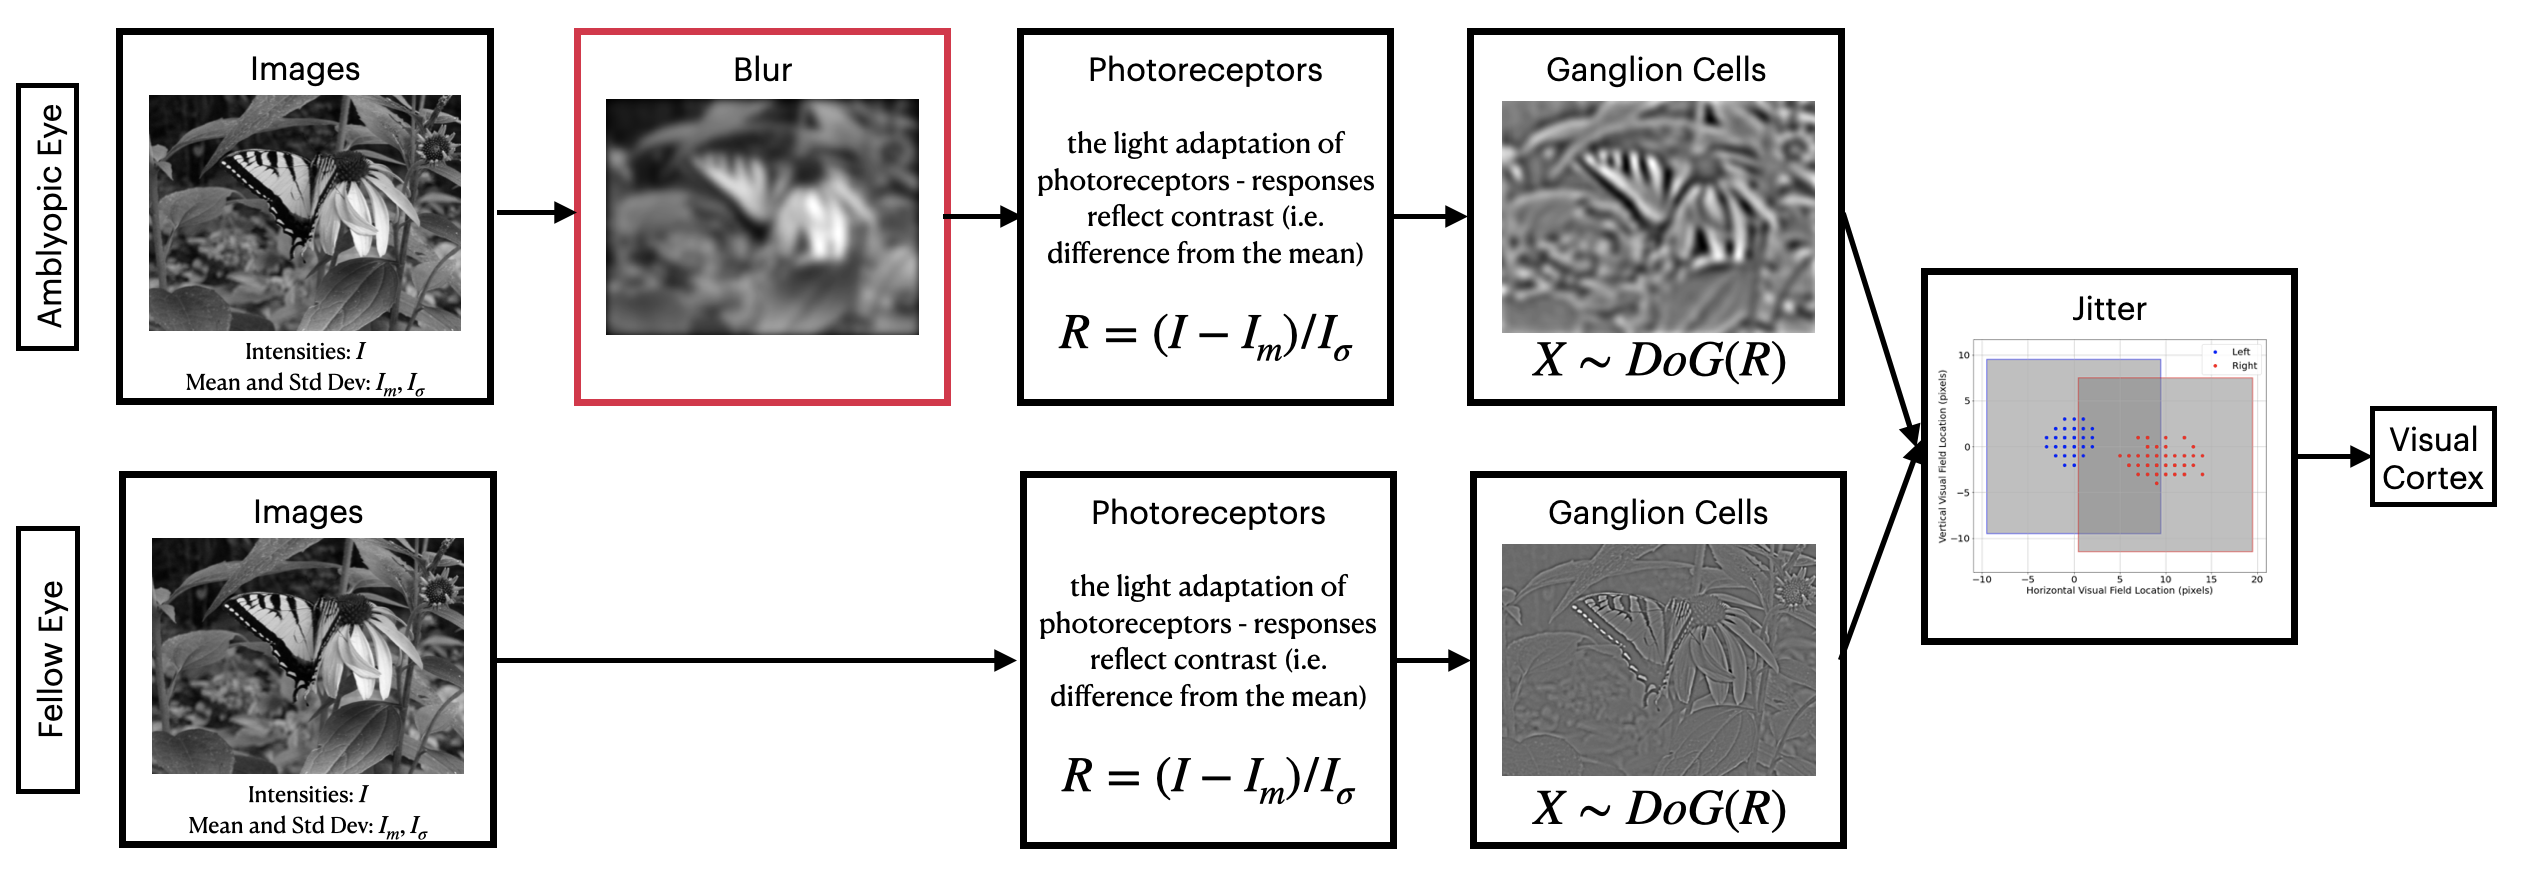
\includegraphics{/Users/bblais/Documents/Git/Amblyopia-Simulation/Manuscript/resources/Pasted image 20240301091305.png}
\caption{Vision Deficit
Model.}\label{fig:Pasted_image_20240301091305.png}
\end{figure}

\begin{figure}
\centering
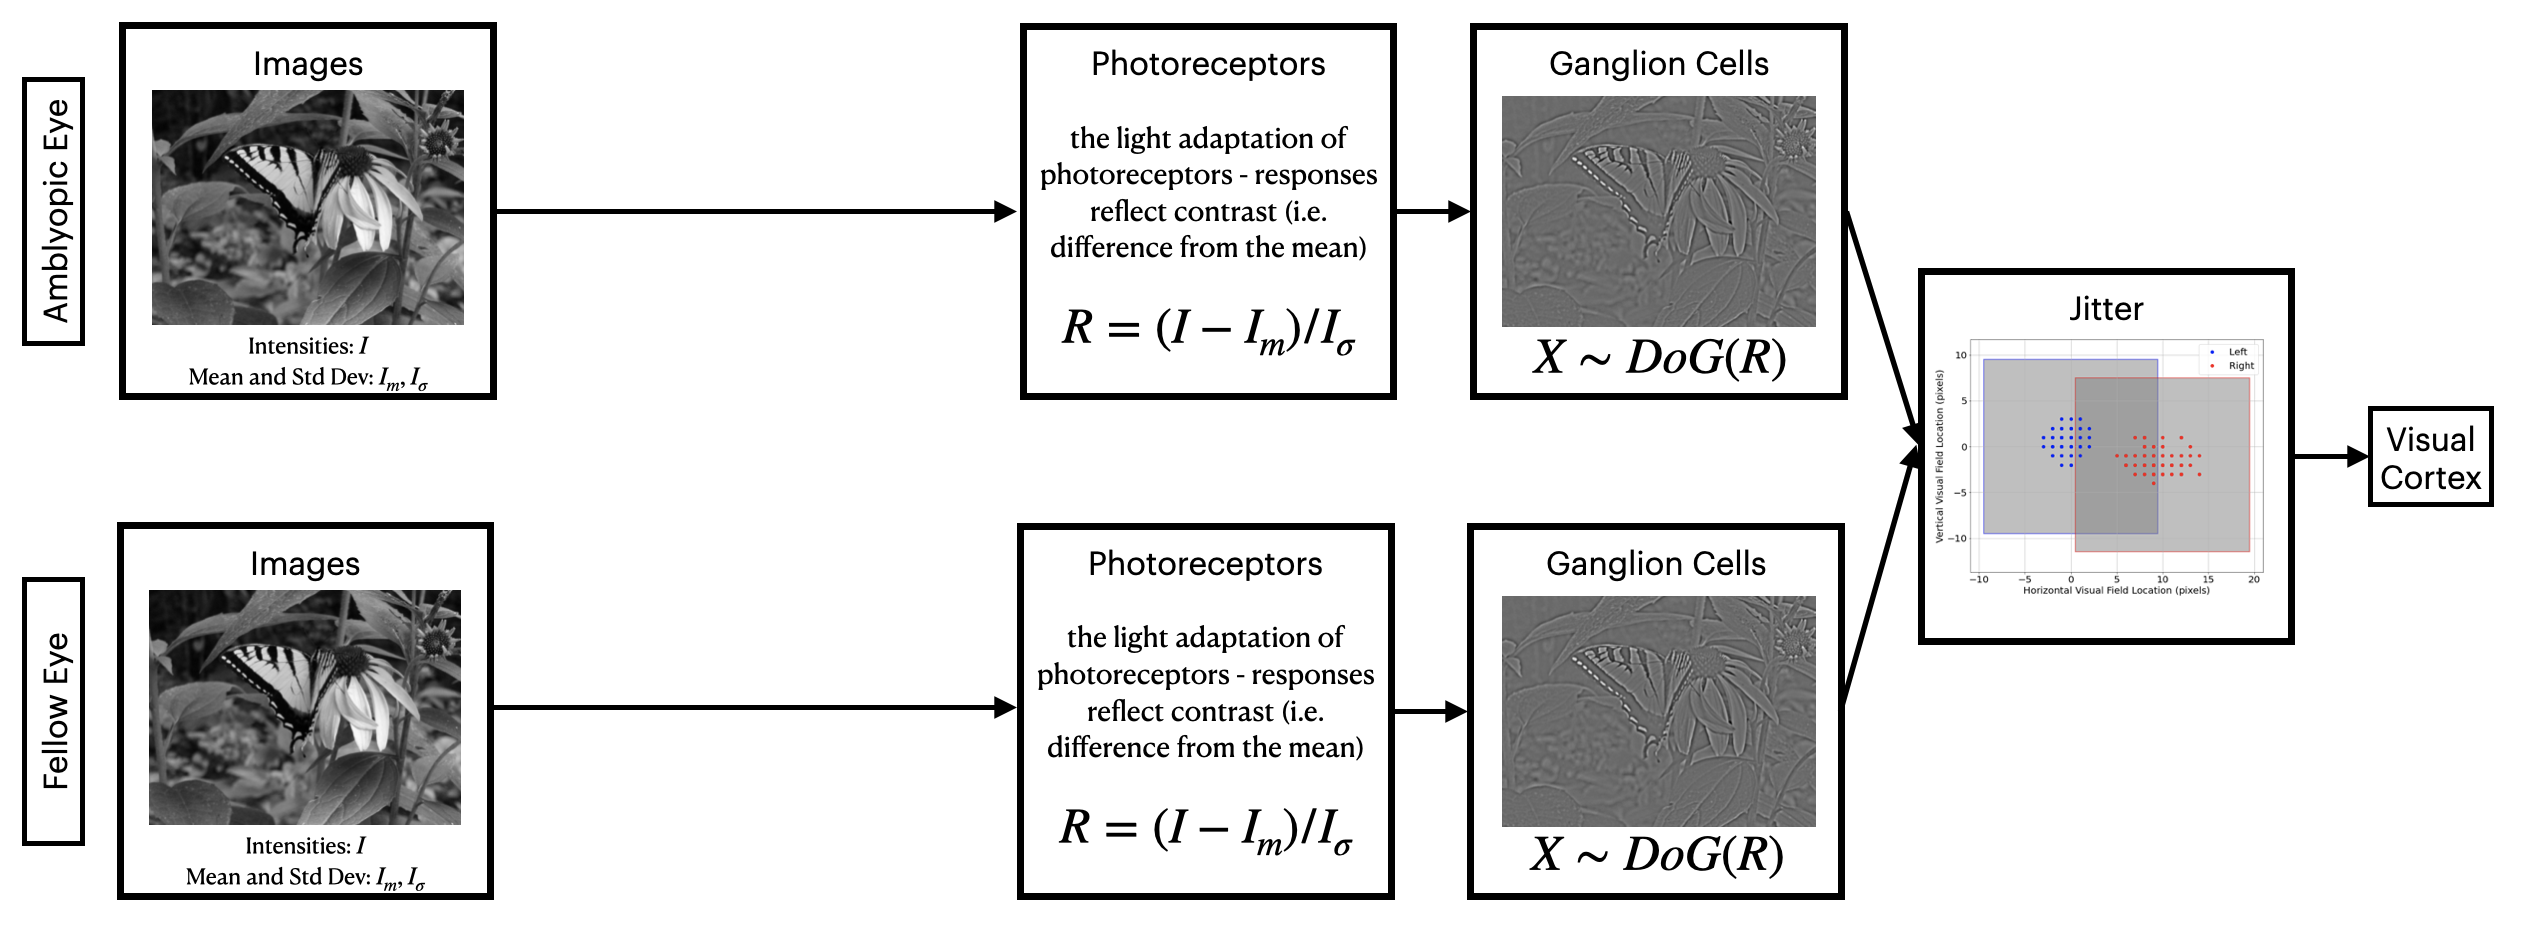
\includegraphics{/Users/bblais/Documents/Git/Amblyopia-Simulation/Manuscript/resources/Pasted image 20240301091503.png}
\caption{Optical Fix Model.}\label{fig:Pasted_image_20240301091503.png}
\end{figure}

\begin{figure}
\centering
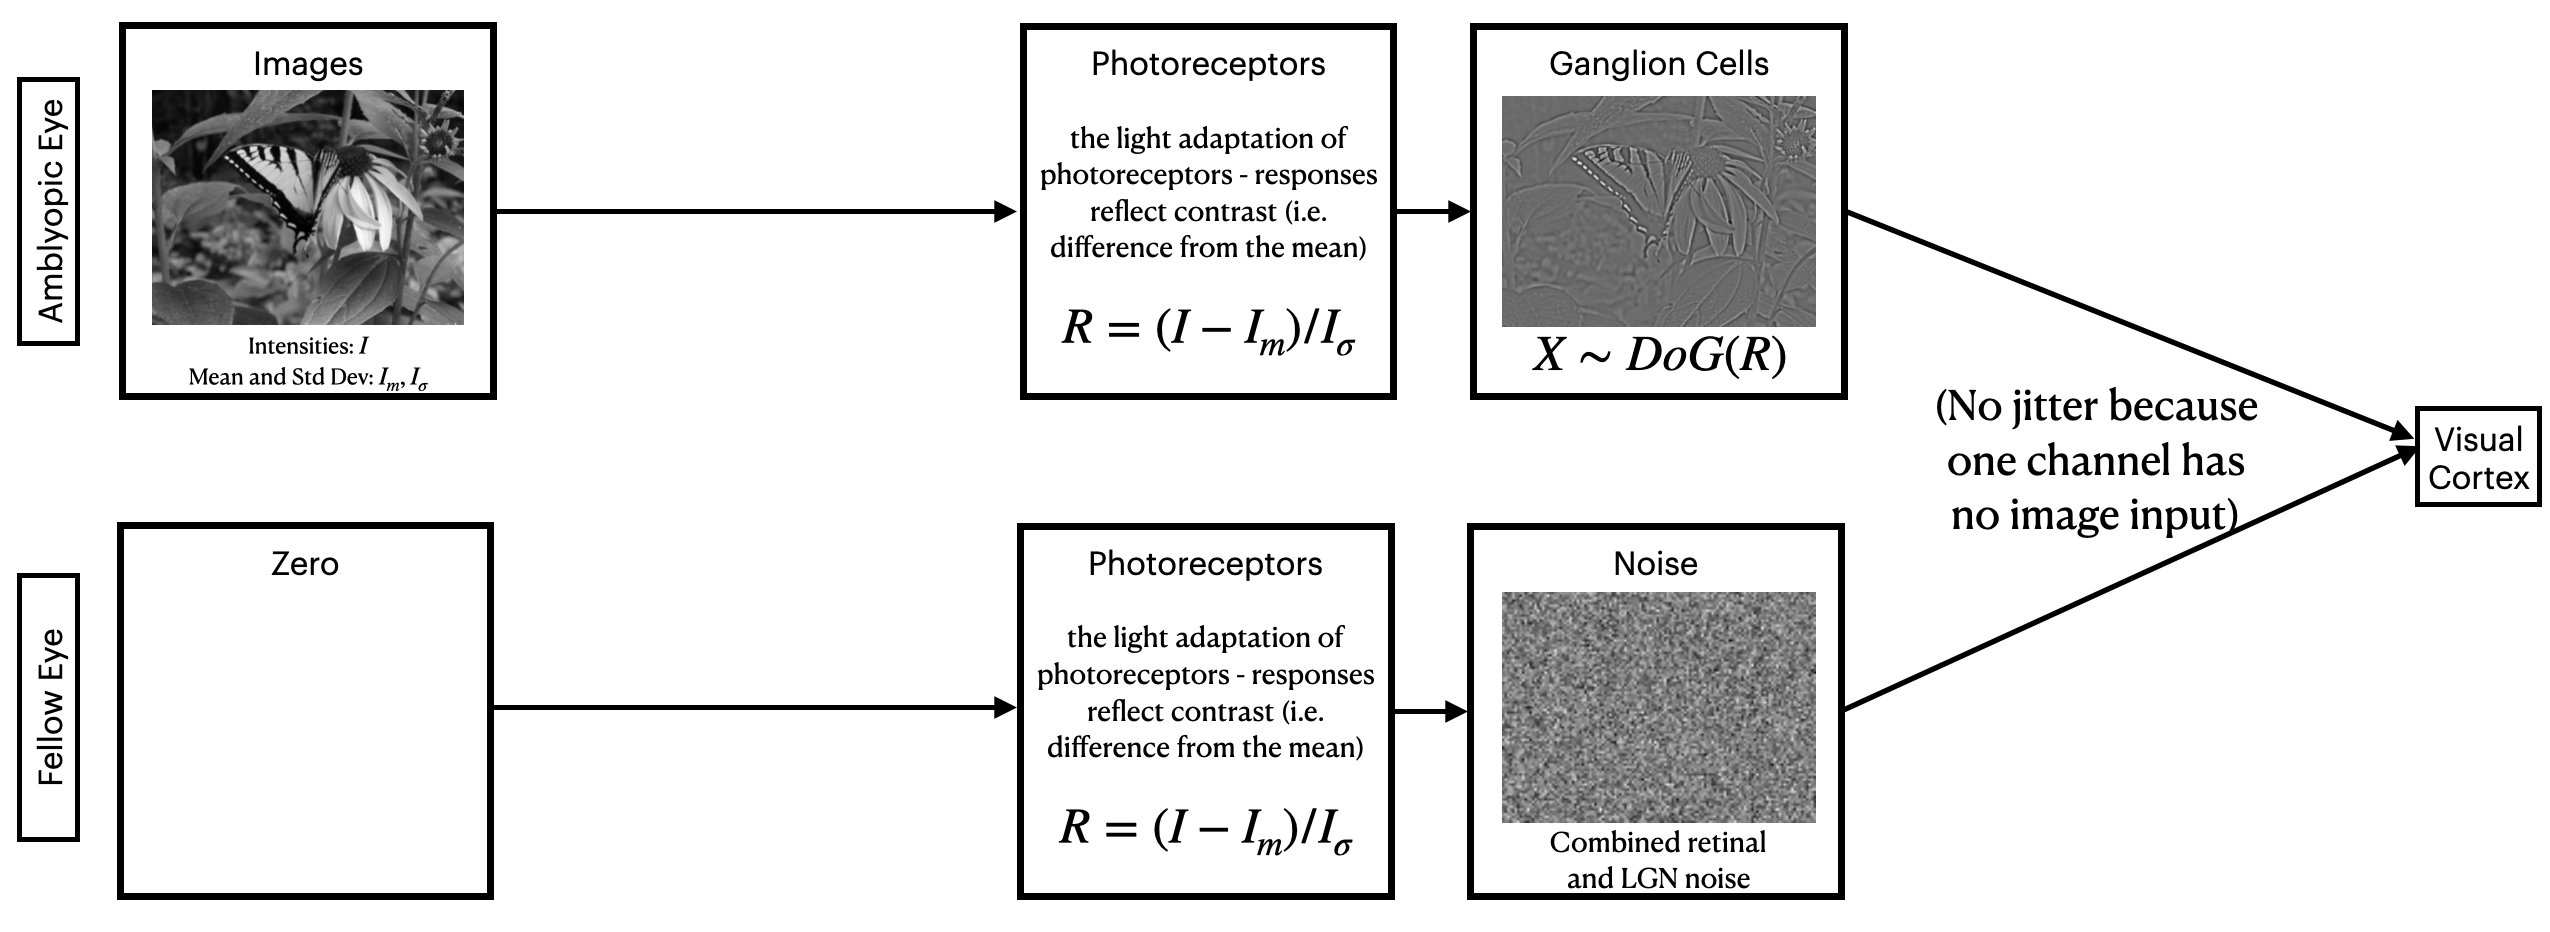
\includegraphics{/Users/bblais/Documents/Git/Amblyopia-Simulation/Manuscript/resources/Pasted image 20240301091523.png}
\caption{Patch Model.}\label{fig:Pasted_image_20240301091523.png}
\end{figure}

\begin{figure}
\centering
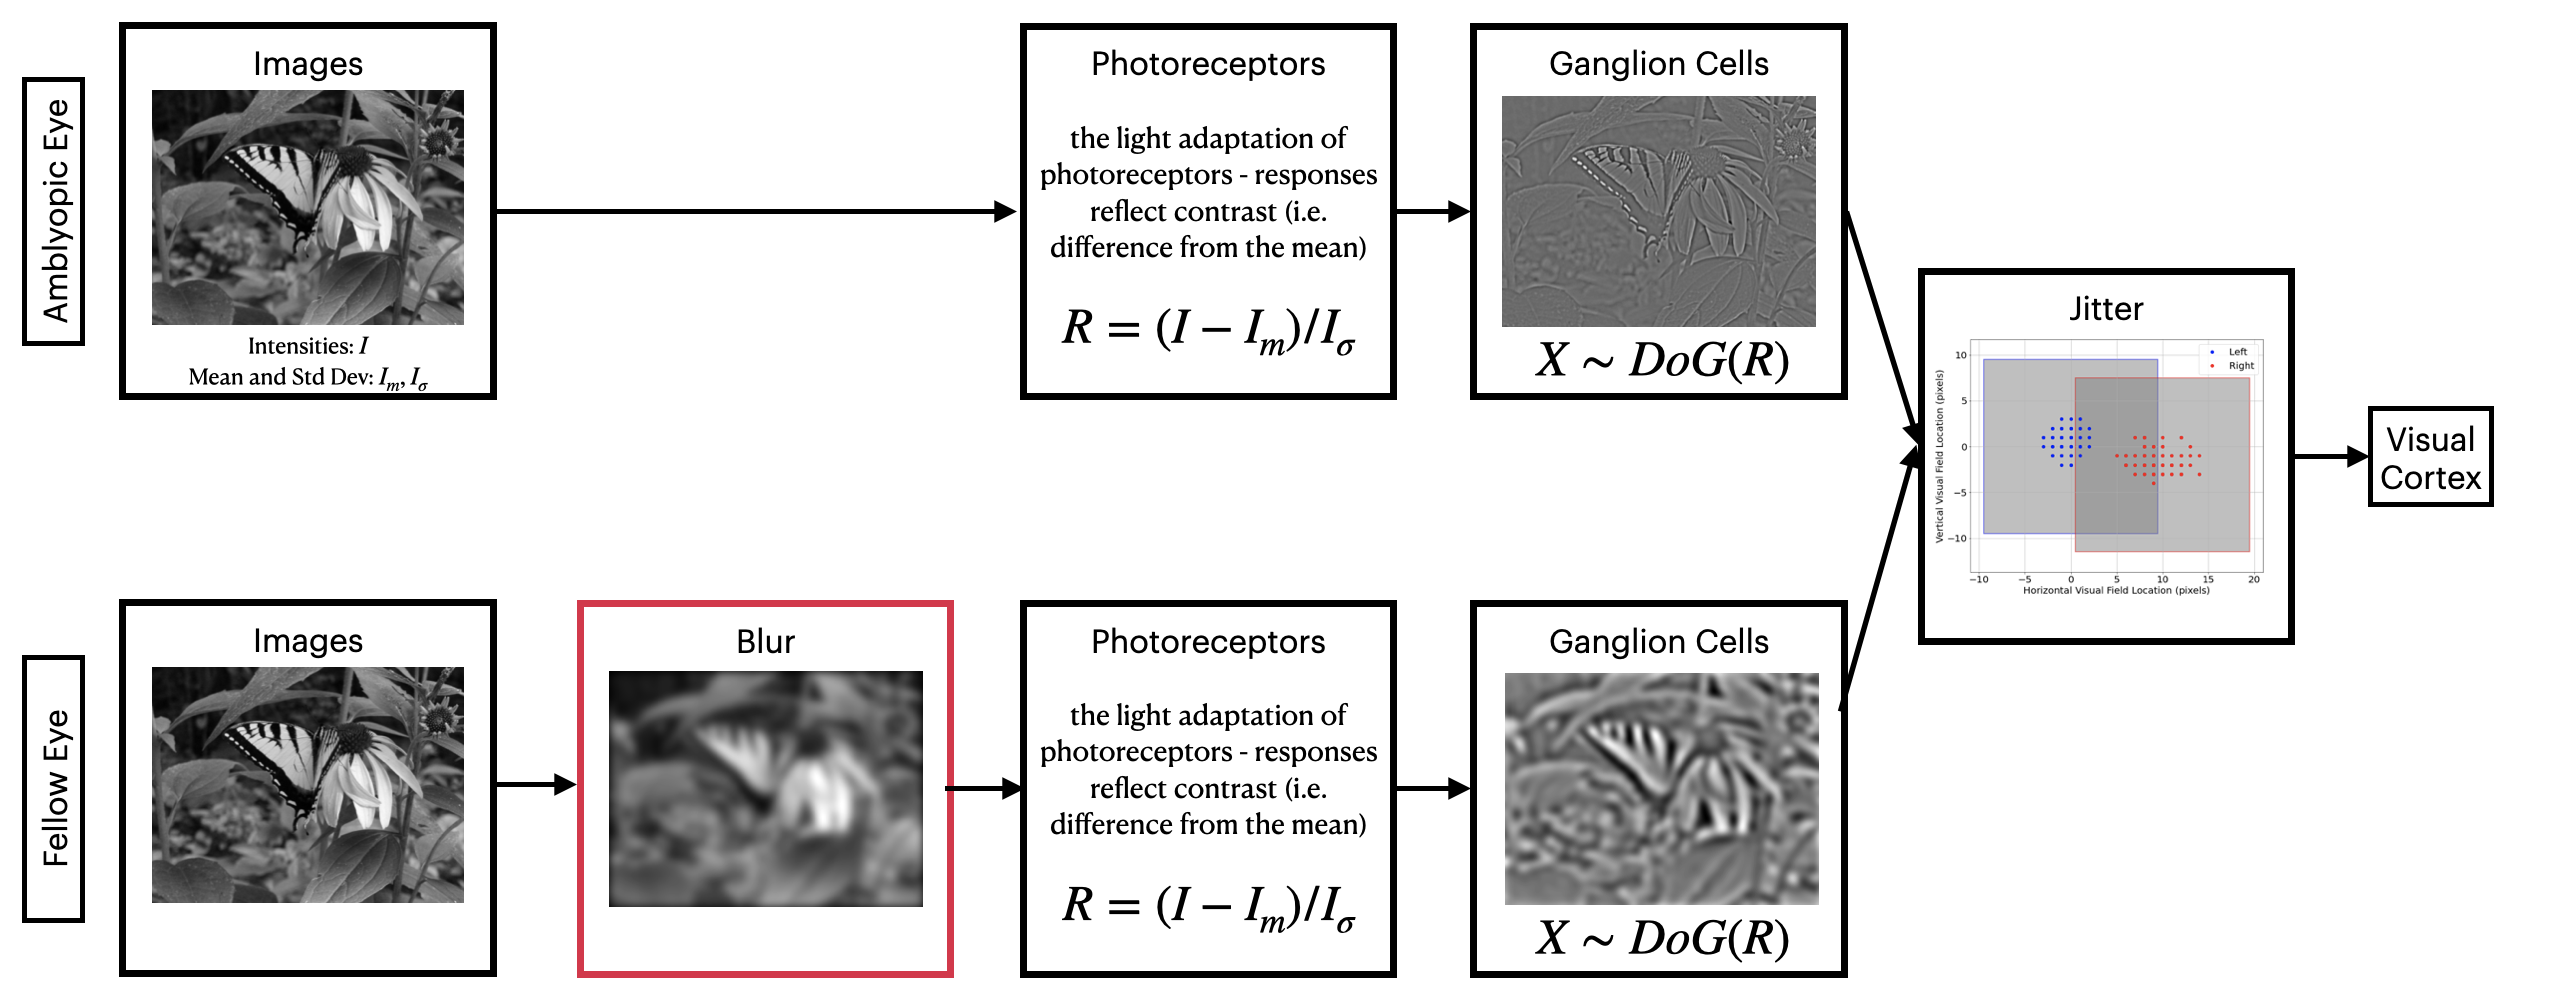
\includegraphics{/Users/bblais/Documents/Git/Amblyopia-Simulation/Manuscript/resources/Pasted image 20240301091538.png}
\caption{Atropine Model.}\label{fig:Pasted_image_20240301091538.png}
\end{figure}

\begin{figure}
\centering
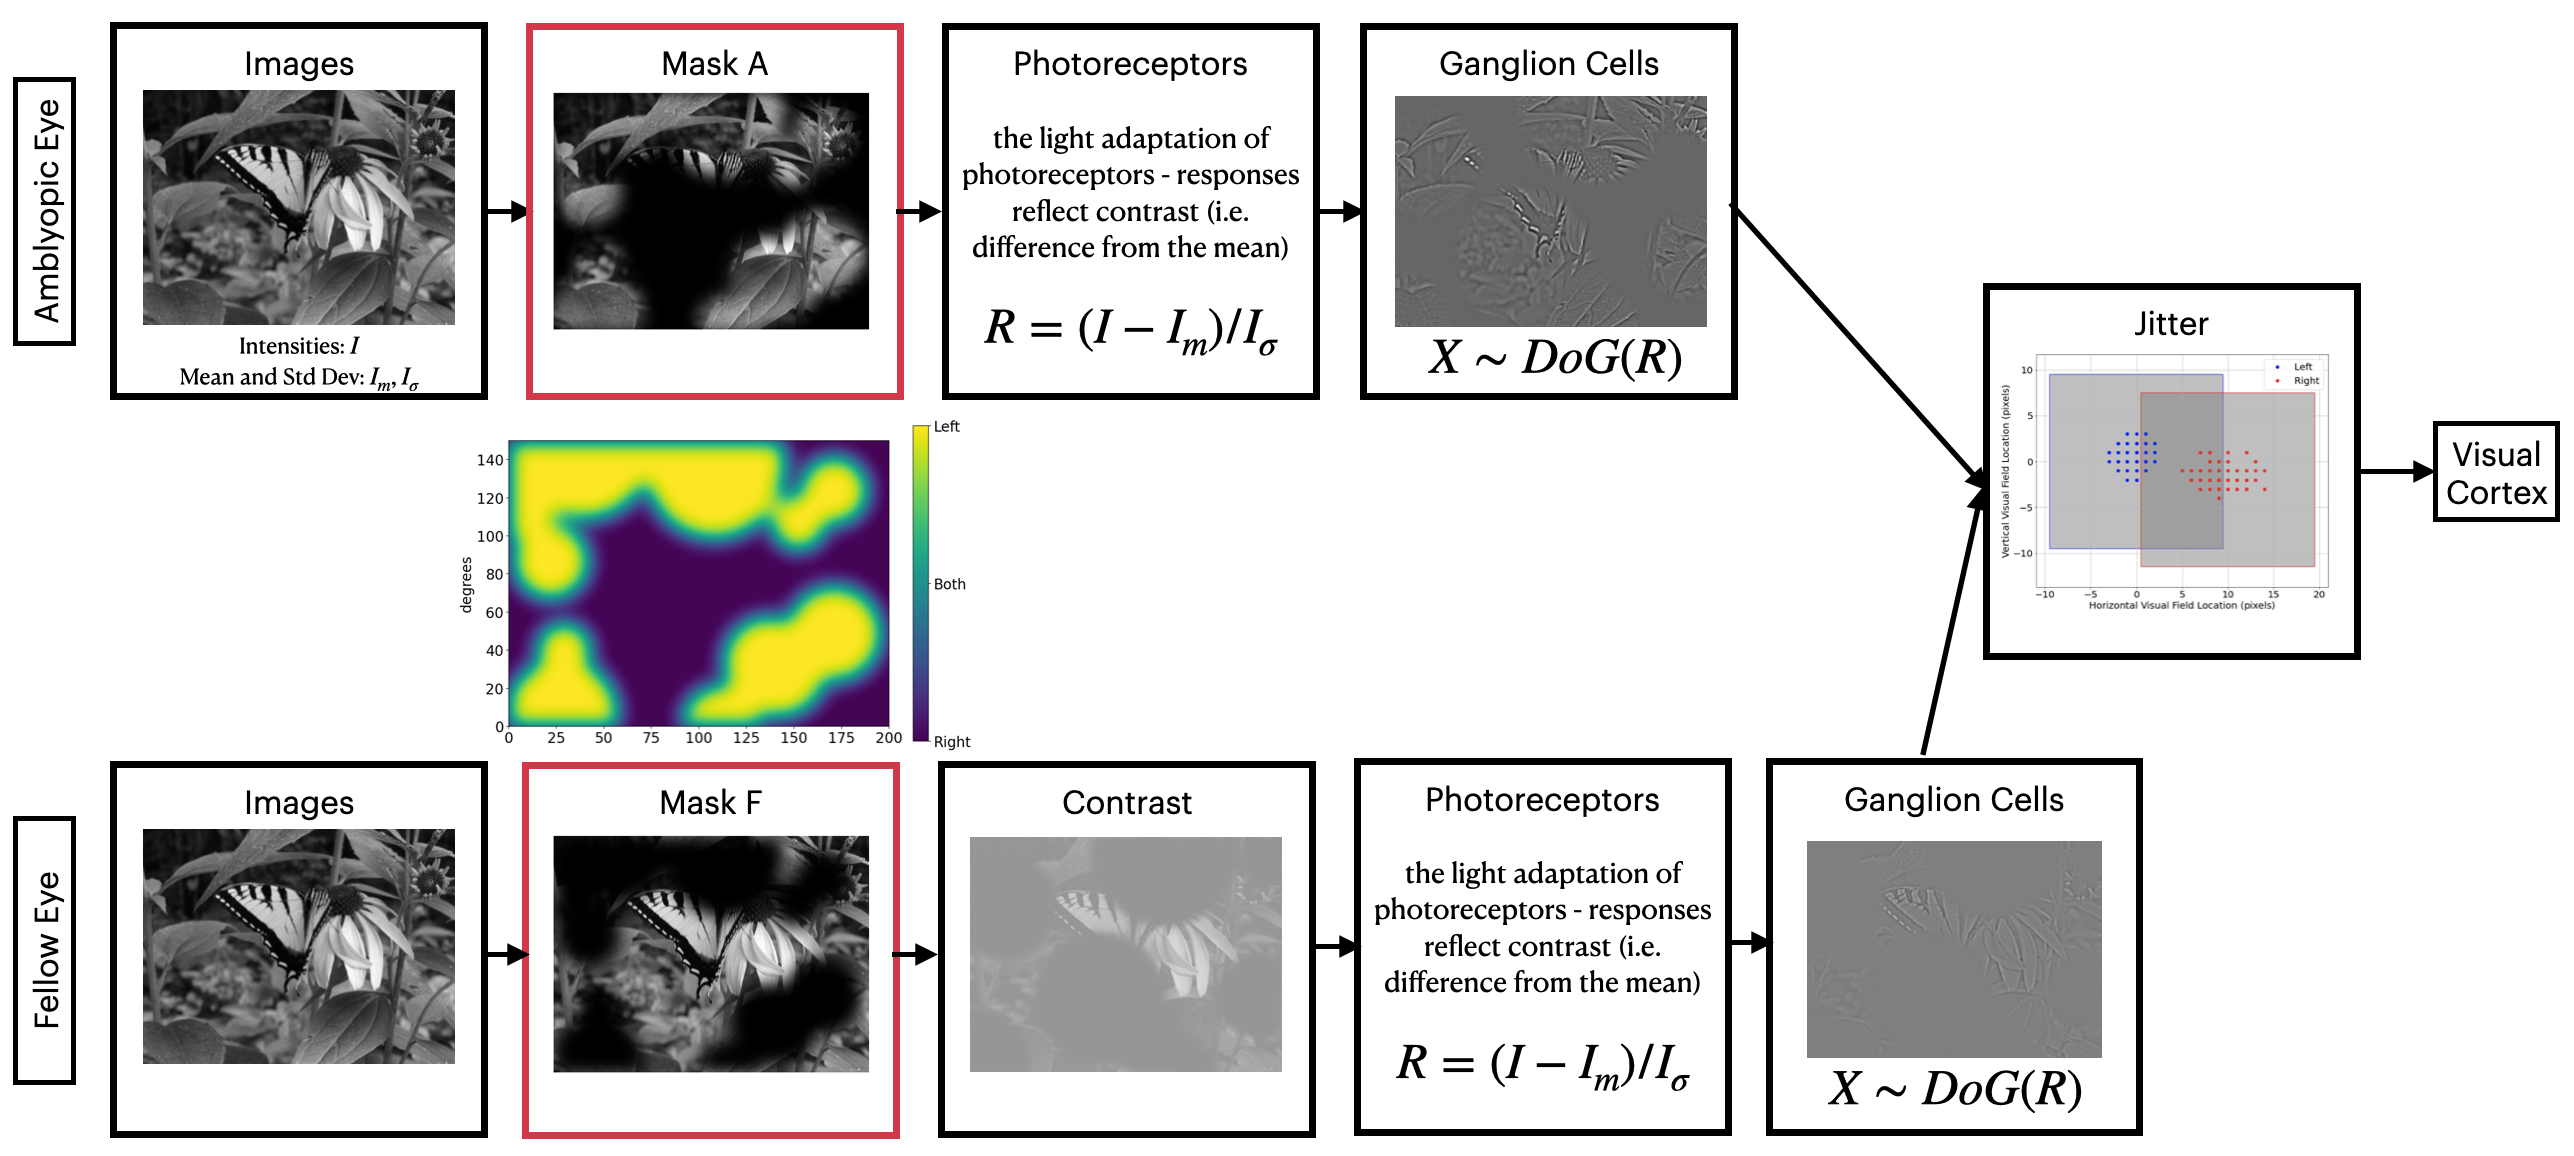
\includegraphics{/Users/bblais/Documents/Git/Amblyopia-Simulation/Manuscript/resources/Pasted image 20240301091600.png}
\caption{Contrast/Mask
Model.}\label{fig:Pasted_image_20240301091600.png}
\end{figure}

\section*{References}\label{sec:references}
\addcontentsline{toc}{section}{References}

\phantomsection\label{refs}
\begin{CSLReferences}{0}{1}
\bibitem[\citeproctext]{ref-BCM82}
\CSLLeftMargin{1. }%
\CSLRightInline{Bienenstock, E.L., Cooper, L.N., and Munro, P.W. (1982).
Theory for the development of neuron selectivity: Orientation
specificity and binocular interaction in visual cortex. Journal of
Neuroscience \emph{2}, 32--48.}

\bibitem[\citeproctext]{ref-phd:Blais98}
\CSLLeftMargin{2. }%
\CSLRightInline{Blais, B.S. (1998). The role of the environment in
synaptic plasticity:\\
towards an understanding of learning and memory.}

\bibitem[\citeproctext]{ref-IntratorCooper92}
\CSLLeftMargin{3. }%
\CSLRightInline{Intrator, N., and Cooper, L.N. (1992).
\href{ftp://cns.brown.edu/nin/papers/cooper.ps.Z}{Objective function
formulation of the {BCM} theory of visual cortical plasticity:
Statistical connections, stability conditions}. Neural Networks
\emph{5}, 3--17.}

\bibitem[\citeproctext]{ref-LawCooper94}
\CSLLeftMargin{4. }%
\CSLRightInline{Law, C., and Cooper, L. (1994). Formation of receptive
fields according to the {BCM} theory in realistic visual environments.
Proceedings National Academy of Sciences \emph{91}, 7797--7801.}

\bibitem[\citeproctext]{ref-brito2024learning}
\CSLLeftMargin{5. }%
\CSLRightInline{Brito, C.S.N. de, and Gerstner, W. (2024). Learning what
matters: Synaptic plasticity with invariance to second-order input
correlations. PLOS Computational Biology \emph{20}, e1011844.}

\bibitem[\citeproctext]{ref-BlaisEtAl99}
\CSLLeftMargin{6. }%
\CSLRightInline{Blais, B., Shouval, H., and Cooper, L.N. (1999). The
role of presynaptic activity in monocular deprivation: Comparison of
homosynaptic and heterosynaptic mechanisms. Proc. Natl. Acad. Sci.
\emph{96}, 1083--1087.}

\end{CSLReferences}

\end{document}
